\documentclass[preprint,3p,onecolumn,times,review]{article}
%\documentclass[preprint,3p,onecolumn,times,review]{elsarticle}
%\documentclass[preprint,3p,twocolumn,times]{elsarticle}
\usepackage[cmex10]{amsmath}
\usepackage{amssymb}
\usepackage{amsfonts}

\usepackage{graphicx}
\usepackage{bussproofs}
\usepackage{booktabs}
\usepackage{soul}
\usepackage{color}
\soulregister\cite7
\soulregister\ref7
\newcommand{\removed}[1]{\st{#1}}
\usepackage{subfigure}
\usepackage{listings}
\usepackage{fancyvrb}
\usepackage{stmaryrd}

\renewcommand{\theenumi}{(\roman{enumi})}

\title{An analysis of structural interoperability \\in {ISO 13606} based on typed lambda calculus}

% \author[plan]{Akimichi Tatsukawa\corref{cor1}}
% \ead{akimichi.tatsukawa@gmail.com}
% \address[plan]{Department of Planning, Information and Management, The University of Tokyo Hospital, Tokyo, Japan.}

% \author[disease]{Emiko Shinohara}
% \address[disease]{Center for Disease Biology and Integrative Medicine, Graduate School of Medicine, The University of Tokyo, Tokyo, Japan.}
% \author[plan]{Takeshi Imai}
% \author[plan]{Yoshimasa Kawazoe}
% \author[plan]{Kazuhiko Ohe}

% \cortext[cor1]{Corresponding author. Address: Department of Planning, Information and Management, The University of Tokyo Hospital, 7-3-1 Hongo, Bunkyo-ku, Tokyo, Japan, Fax: +81 3 3813 7238\\
% \qquad Email address: akimichi.tatsukawa@gmail.com}

\newtheorem{thm}{Theorem}
\newtheorem{lem}[thm]{Lemma}
%\newdefinition{rmk}{Remark}
%\newproof{pf}{Derivation}
\newcommand{\HL}[1]{\hl{\mbox{#1}}}

\begin{document}

\maketitle

%\begin{frontmatter}

\begin{abstract}
  ISO 13606 defines a standard specification for the exchange and integration of electronic health record (EHR) data with the goal of interoperability of EHR data across heterogeneous systems.
  In order to achieve this goal, the ISO 13606 standard provides a dual-model architecture in which archetypes are extensible schemas of EHR data via their specialization and composition mechanisms.
  However, the ISO 13606 standard lacks the formal semantics of archetypes, which makes it difficult to build EHR systems or archetype repositories in a consistent and longitudinal manner.
  The goal of the present study was to clarify the archetype semantics of ISO 13606 by means of a formal methodology called typed lambda calculus, which has been widely used to define and analyze the semantics of modern programming languages and database systems.
  We focus on the variance and immutability of the archetype, because these factors determine the expressive power of archetypes.
  We defined a type system that represents the fundamental components of ISO 13606 semantics and analyzed the semantics based on a deductive system of the type theory.
  The obtained results indicate that the archetypes should be covariant and immutable schemas in order to guarantee both the structural interoperability of EHR data and the extensibility of archetypes.
\end{abstract}



% \begin{keyword}
%    ISO 13606 \sep Archetypes \sep Typed Lambda Calculus \sep Formal Semantics \sep openEHR
% \end{keyword}

%\end{frontmatter}

%\tableofcontents

\section{Introduction}

\subsection{Background}

The efficient use of medical resources and the fulfillment of large-scale clinical research requires integration of electronic healthcare record (EHR) systems that store diverse clinical data for long periods of time.
This challenge, however, remains unsolved even today.
The heterogeneity of these data sources, i.e., the interoperability of EHR data from local systems in a consistent and longitudinal manner, is a major obstacle for the integration or exchange of data across EHR systems \cite{sujansky01:_heter}.
In order to achieve interoperability, the schema of EHR data must satisfy the requirements of various organizations and evolve over time in accordance with the development of medical domains.

ISO 13606 standard defines a common healthcare model for such a purpose.
The overall goal of the standard is "to devise a generalized approach representing every conceivable kind of health record data structure in a consistent way" \cite[vi]{iso08:13606_healt_elect_part1} so as to "support the interoperability of systems and components that need to communicate EHR data" \cite[v]{iso08:13606_healt_elect_part1}.
Due to the complexity and continuing evolution of the healthcare domain, the common model must meet the needs of organizations and cope with the progress of medical domains.
In order to overcome these difficulties, ISO 13606 has adopted a dual-model approach that distinguishes two modeling layers, i.e., information layer and knowledge layer, which are explained later.

While this dual-model architecture is a major feature of ISO 13606, the  original idea stems from the openEHR specification, which was also an attempt at the "sharing of EHRs via interoperability at data and knowledge levels" \cite[p.12]{beale08:_openeh_archit_overv}.
In fact, ISO 13606 is largely considered to be a subset of the full openEHR specification \cite{peter:_relationship_cen13606_hl7_openehr,chen09:_archet_conversion_ehr_model}. Therefore, both specifications share common features.
The present paper refers primarily to ISO 13606 as a standard for the interoperability of EHR systems. However, for the case in which ISO 13606 is short of sufficient descriptions and the openEHR specification is more appropriate, we will refer to the openEHR specification as a secondary resource.

As specifications become larger and more complicated, the consistency and correctness of the specifications become uncertain, and ISO 13606 is no exception.
The ISO 13606 specification describes the behavior of archetypes but does not define any formal semantics.
This is problematic because the lack of a formal definition makes the implementation of an EHR system difficult.
For example, when we define an archetype using both specialization and composition, are we allowed to combine them in an arbitrary manner? Or, are there constraints embedded in the semantics of the archetypes?
These questions have to be answered before the design and implementation of an EHR system.

Since ISO 13606 provides insufficient explanation regarding these questions, we must look back at the original openEHR specifications for clues.
In the two specifications, we found two important statements. One is cited from the ISO 13606 specification, and the other from the openEHR specification.

\begin{enumerate}
\item Assertion 1

  Any data created via the use of a specialized archetype shall be conformant to both the archetype and its parent \cite[viii]{iso08:13606_healt_elect_part2}.
\item Assertion 2

  Data created with any specialized archetype will always be matched by queries based on the parent archetype \cite[p.51]{beale08:_openeh_archit_overv}.
\end{enumerate}

These assertions are prerequisites for laying the groundwork on archetype semantics, because they suggest the requirements for EHR data conformance and queries based on archetype.
However, the exact meanings remain unclear because natural language descriptions leave room for a wide range of interpretations.
For example, what does the phrase 'conformant to' mean exactly? How can we assure that certain queries match appropriate EHR data and that others do not?

\subsection{Objective}


The goal of the present study is to clarify the ISO 13606 archetype semantics in order to support the two assertions above. We investigate the semantics in a formal manner under the assumption that at least these two assertions must hold, and we pursue further consequences that are logically derived from the semantics.
The term 'formal methodology' refers to the situation in which every term in a syntax or every property in semantics is defined by a symbol so that each has a precise meaning that serves as a foundation for reasoning or verification. 


As a means of such formalization, we used {\bf typed lambda calculus}, which is widely used as meta-language in the field of computer science to define and analyze the semantics of various programming languages and database systems \cite{ohori89:_simpl_seman_ml_polym,igarashi01:_feath_java}.
We believe that this formalization technique can contribute to the analysis of ISO 13606 in the same manner as previous domains in computer science.
To the best of our knowledge, this is the first attempt to apply typed lambda calculus to semantics in the medical field.

\section{Material and Methods}


\subsection{Concepts for EHR data integration\label{sec:higher_concepts}}

Even if a formal methodology is necessary for building a solid semantics, it is not sufficient.
When we encounter different results from different premises, we must choose one of the results based on higher conceptual criteria, even though these results are both valid in terms of formalization.
Before introducing the formal methodology of typed lambda calculus, we begin by explaining several fundamental concepts for the exchange and integration of EHR data.
These concepts are 'structural interoperability' and 'schema extensibility'.


\subsubsection{Structural interoperability should be guaranteed}


Every standardization of clinical information, including ISO 13606, attempts to achieve a certain level of interoperability between EHR systems.
ISO 13606 defines 'interoperability' as the "ability for data shared by systems to be understood at the level of fully defined domain concepts" \cite[p.5]{iso08:13606_healt_elect_part1}.
However, the term 'to be understood' is not precise in terms of computer science. Computers can never 'understand' the meaning of data, they only compute.
Moreover, we believe that this ambiguity has its root in the fact that two different types of concepts are being explained using one term 'interoperability'.
Thus, we divided the concept of interoperability into two levels, as follows.

\begin{enumerate}
\item Structural Interoperability
  
  Structural interoperability is defined as the ability to process data based on a shared formal schema with sound semantics. 
  This type of interoperability is referred to as 'structural' because modern database schemas or data models are solely concerned with the structure of data, such as field names, data types, and relations.
\item Semantic Interoperability

  Semantic interoperability, in contrast, is defined as the ability to process data based on the shared meanings of terms \cite{veltman01:_syntac_seman_inter,sebastian09:_towar_seman_inter_for_elect_healt_recor,maldonado07:_framew_for_clinic_data_stand_based_archet,martinez-costa10:_iso_en_openeh,jose09:_linkeh_ed}.
  In order to share the meanings of terms, we need mapping between objects in a virtual world (i.e., the computer) and concepts in the real world, because the 'meaning' refers to our interpretation of assignments between concrete objects and abstract concepts \cite[p.97]{hakimpour05:_resol_seman_heter_datab_schem}.
  The concepts in the real world, however, can neither be directly represented nor processed by computer.
  Therefore, the assignments are technically performed both by defining ontologies, which are surrogates for the real world concept, and by annotating terms or attributes with the corresponding items in the ontologies.
\end{enumerate}

\begin{figure*}[!htbp]
  \begin{center}
    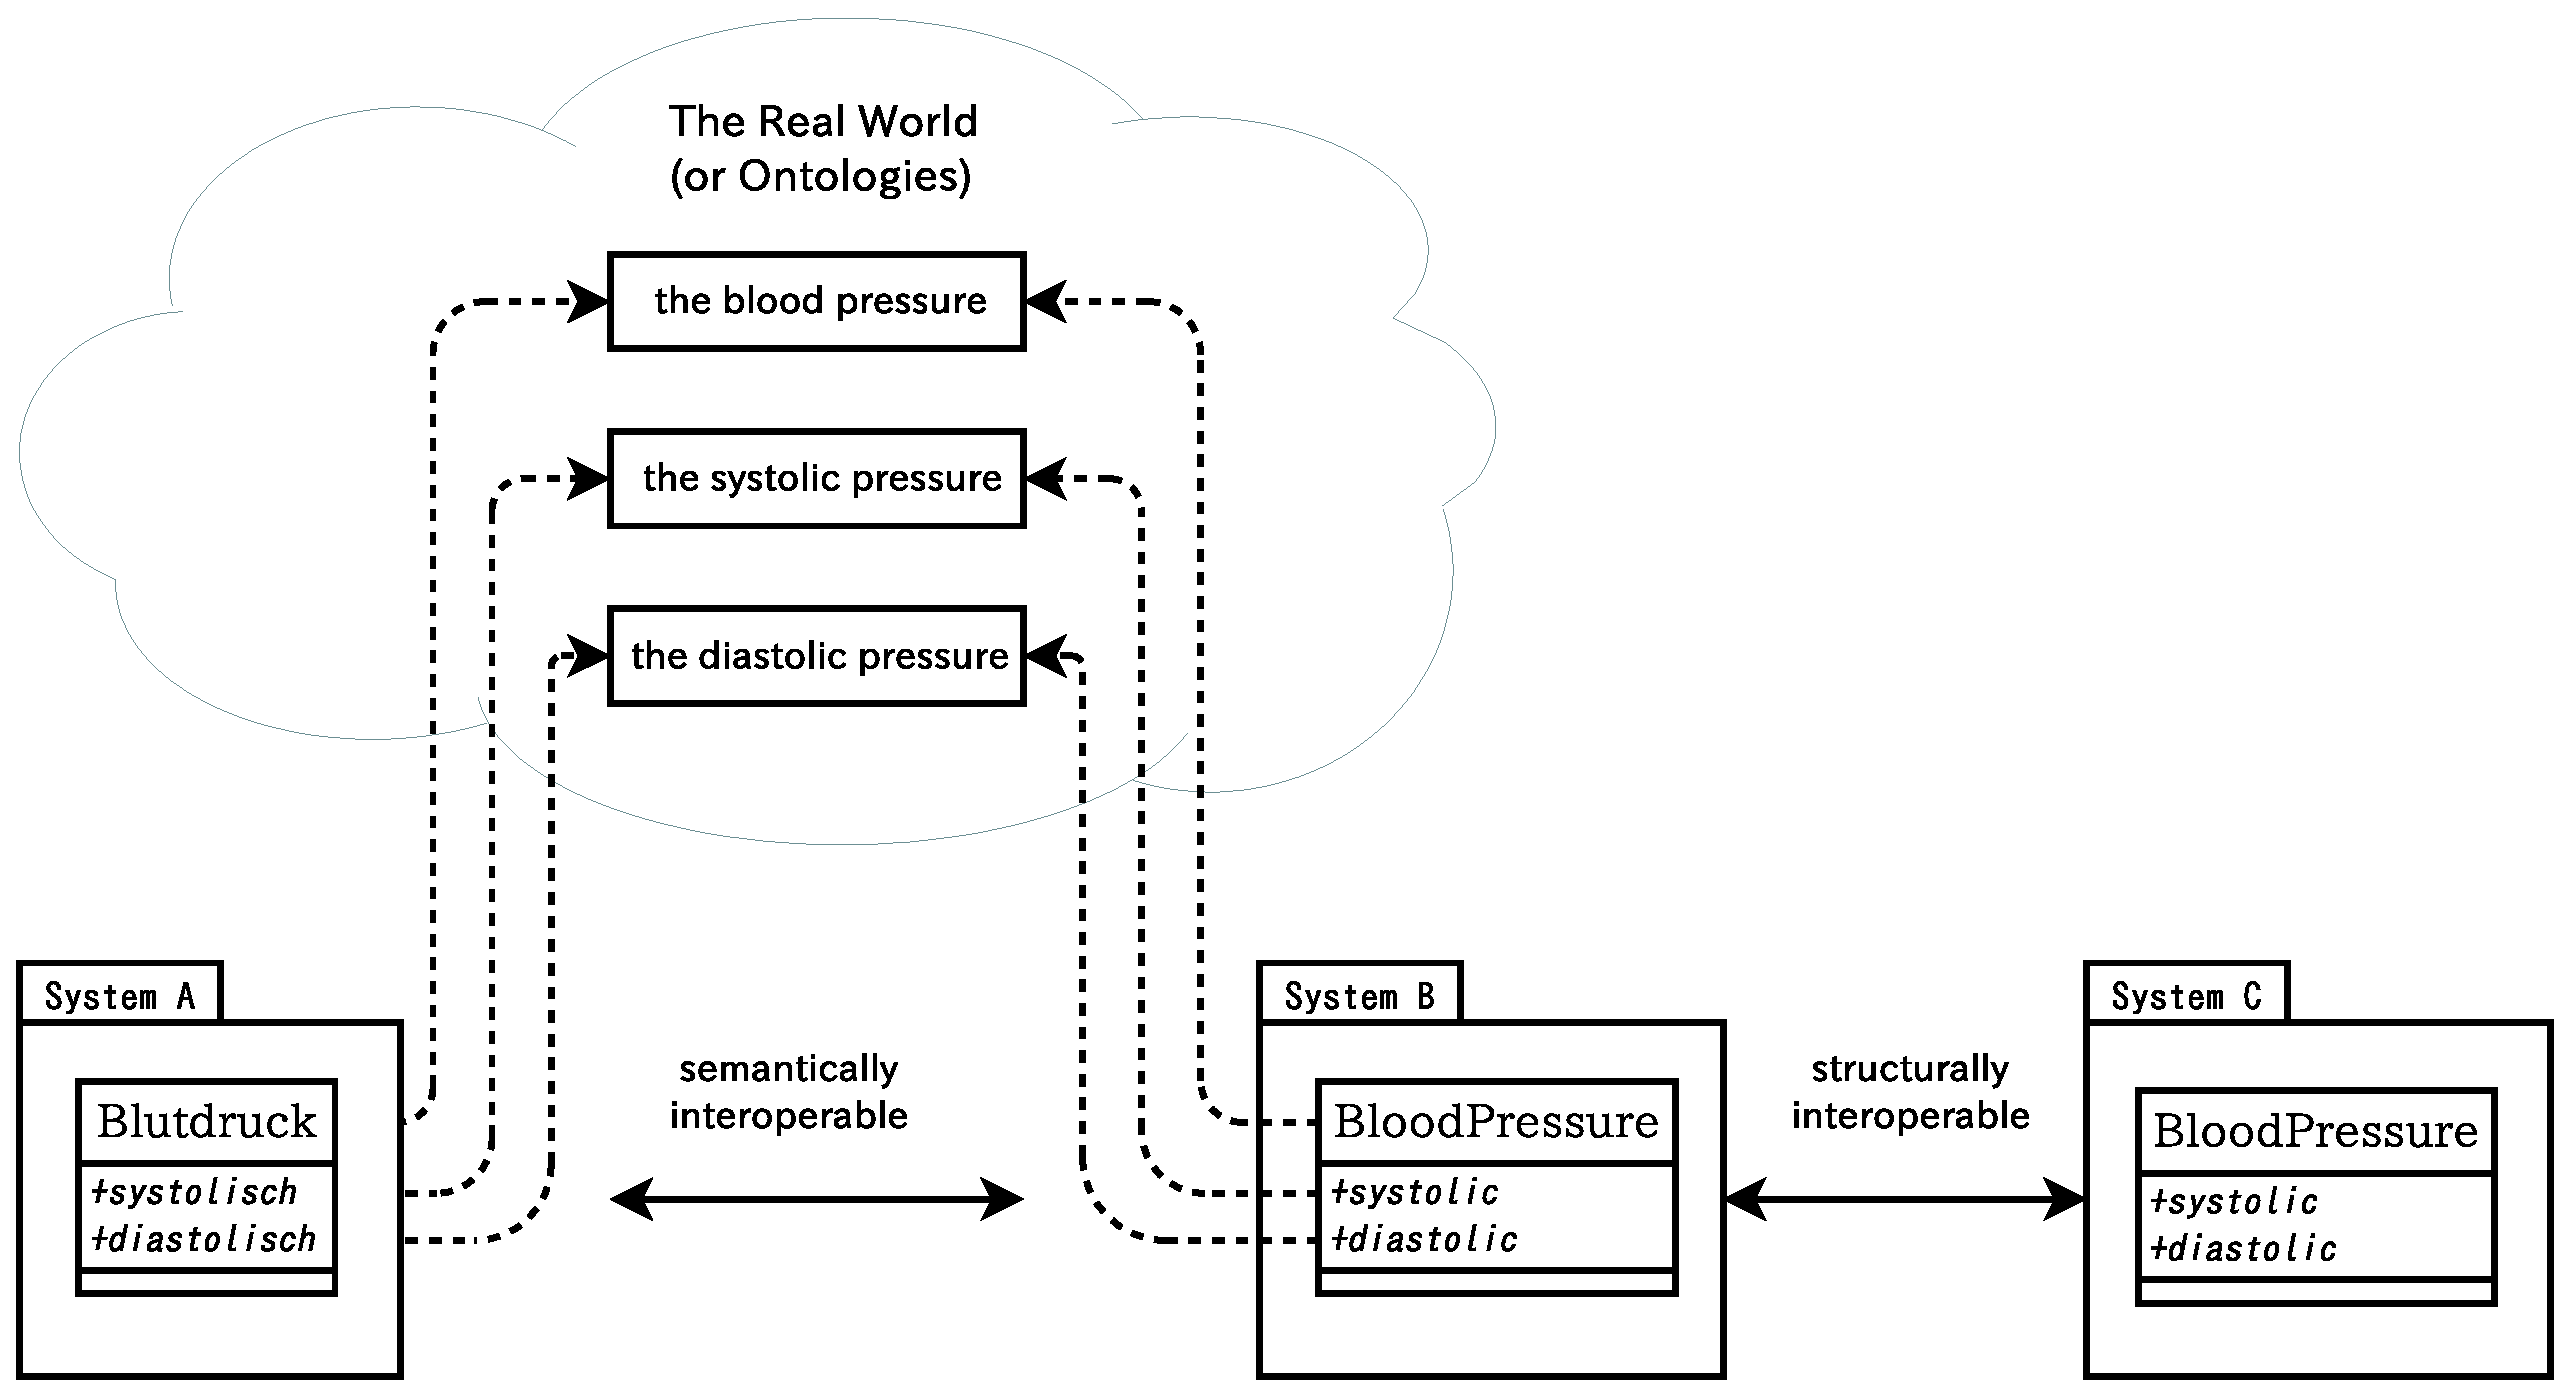
\includegraphics[width=12cm]{meaning_of_semantic.eps}  
  \end{center}
  \caption{Structural interoperability and semantic interoperability}\label{fig:meaning_of_semantic}
\end{figure*}

Figure \ref{fig:meaning_of_semantic} illustrates the difference between structural interoperability and semantic interoperability.
All three EHR systems define blood pressure in their schemas.
Systems B and C have structurally identical schemas and are therefore structurally interoperable.
System A has a different schema from the other systems, because their attribute names are written in German.
As a result, Systems A can be semantically interoperable with System B only if the mapping between the attributes and the real concepts is correctly defined.

Figure {\ref{fig:meaning_of_semantic}} appears to indicate that structural interoperability and semantic interoperability are two independent concepts.
However, structural interoperability is necessary even when semantic interoperability is to be accomplished, because semantic annotations are useful only if the valid values can be obtained without errors. For example, let us think of a situation in which we collect systolic blood pressure data both from Systems A and B in Fig. {\ref{fig:meaning_of_semantic}}. According to the ontology, we get table names (${\mathsf{BloodPressure}}$ and ${\mathsf{Blutdruck}}$) and column names (${\it systolic}$ and ${\it systolisch}$) for each system. Only when we have this structural information can we actually retrieve the data.
Thus, structural interoperability is more fundamental than semantic interoperability.
The present study focuses on the concept of structural interoperability in the investigation of archetype semantics.

\subsubsection{EHR schema should be extensible}

When every EHR system is built upon a unified and fixed EHR schema, we can easily achieve structural interoperability.
In real settings, however, building such a single giant schema is difficult, especially in the medical domain, where concepts are not only large, but also open-ended with respect to breadth, depth, and complexity \cite{rector99:_clinic_termin,renner96:_data_inter}.

The following example, which is a longitudinal cancer cohort study, illustrates the difficulties involved (Fig. \ref{fig:cohort_study}). At the start of the study, we store smoking histories as the exposure level and several tumor markers as surrogates for cancer outcome.
When a novel marker is discovered during the course of the study, we want to add the marker as an additional item, such as {\sf RevisedOutcome} in {\sf RevisedCase} (Fig. \ref{fig:cohort_study}).
Or, if an unexpected exposure, such as a nuclear plant accident, is observed, the extra exposure (in this case, an irradiation dose) should be added.

As this example indicates, when data are stored and traced longitudinally, the EHR schema must be extended as medicine progresses or a new event occurs. Otherwise, a number of disorganized schemas, many of which are similar but slightly different, will accumulate, and the cost of maintenance will increase significantly.


\begin{figure*}[!htbp]
  \begin{center}
    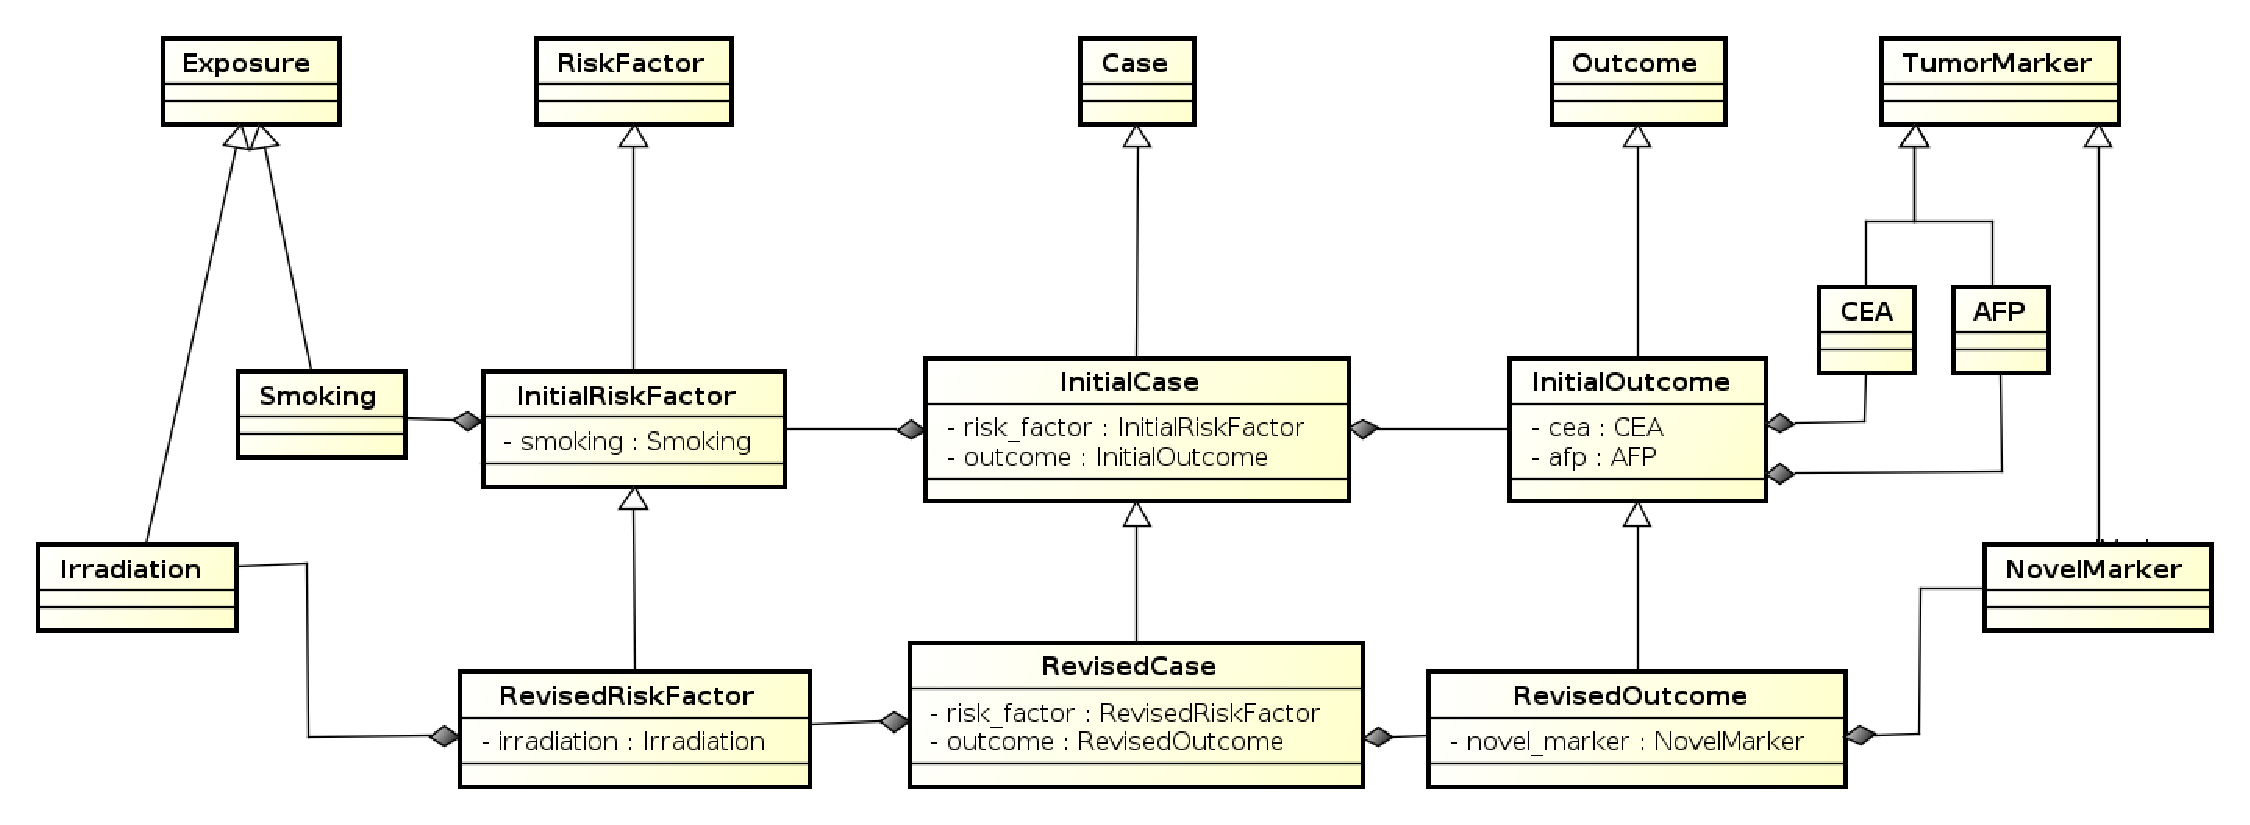
\includegraphics[width=16cm]{cancer_cohort_study_schema.eps}  
  \end{center}
  \caption{Unified Modeling Language (UML) diagram of an imaginary cohort study}\label{fig:cohort_study}
  {\footnotesize
    The diagram describes the schema of an imaginary cohort study in chronological order.
    The lower diagram indicates the more recent content.
    }
\end{figure*}

\subsection{ISO 13606 architecture}

In this section, we present an overview of ISO 13606 in terms of the dual model architecture.
In particular, we focus on the specialization and composition of archetypes.
At the end of this section, we point out the problem associated with their combination (archetype variances).

\subsubsection{Dual-model architecture}


Like openEHR, ISO 13606, adopts a dual-model architecture (Fig. \ref{fig:dual_model_approach}) to guarantee interoperability and support flexibility of archetypes as EHR schema.
The architecture defines a Reference Model (RM) and an Archetype Model (AM) in the lower layer and archetypes in the upper layer, and it proposes building archetypes by constraining RM classes by means of an AM.

\begin{figure}[!htbp]
  \begin{center}
    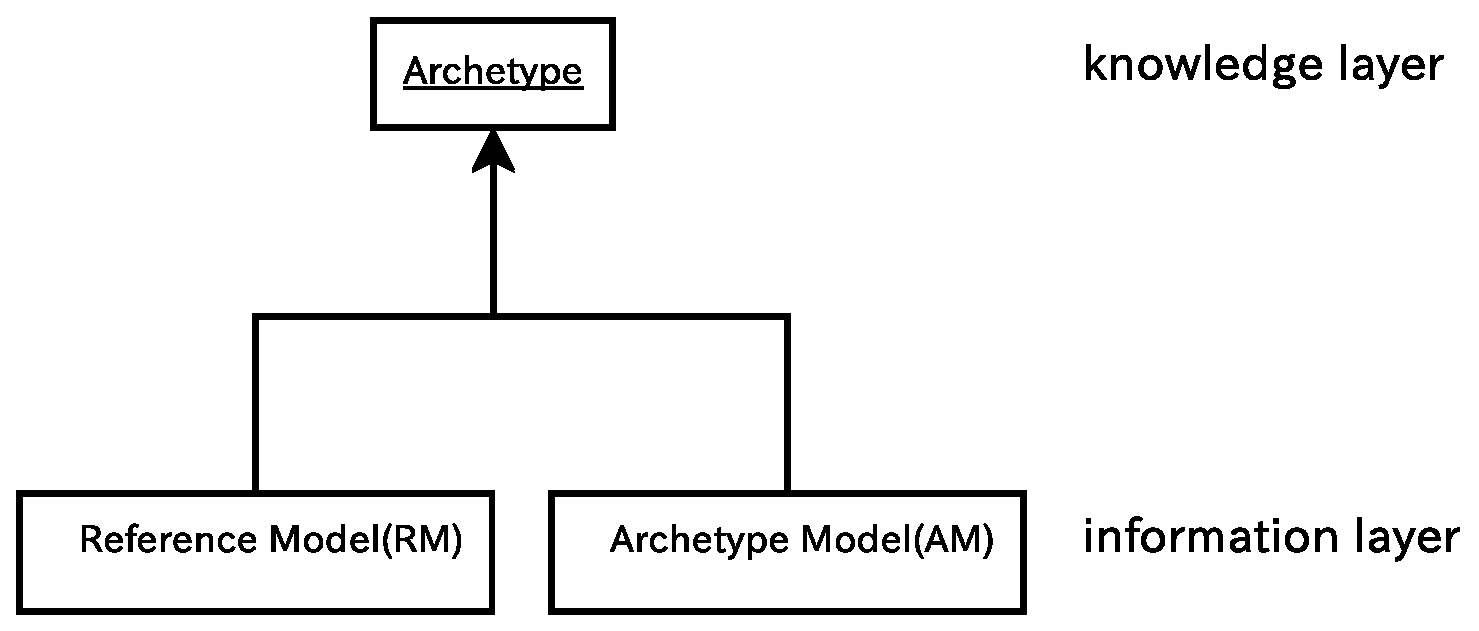
\includegraphics[width=7cm,clip]{dual_model_approach.eps}  
  \end{center}
  \caption{Relationships between RM, AM, and Archetype in the dual model architecture}\label{fig:dual_model_approach}
  {\footnotesize
    The diagram describes the dual-model architecture of ISO 13606, which consists of two layers, an information layer and a knowledge layer. The lower side of the figure indicates the information layer, in which the Reference Model and the Archetype Model are located, and the upper side indicates the knowledge layer, in which the Archetype resides.}
\end{figure}


The lower layer of the dual-model architecture contains a Reference Model and an Archetype Model.
The {\bf Reference Model} defines a set of data structures and data types from which any health record information is composed \cite[p.vi]{iso08:13606_healt_elect_part1}.
Sitting in the lower layer of the dual-model architecture, the RM represents the generic properties of health record information \cite[p.vi]{iso08:13606_healt_elect_part1} , and forms the generic building blocks of the EHR.

The {\bf Archetype Model} also sits in the lower layer, and acts as a skeleton or template for archetypes.
The model consists of "identifying information, a description (its metadata), a definition (expressed in terms of constraints on instances of an object model), and an ontology" \cite[p.vii]{iso08:13606_healt_elect_part2}.
The definition section defines the hierarchical organization of a set of nodes and constraints on the permitted values of attributes and data values \cite[p.6]{iso08:13606_healt_elect_part2}.
In other words, the AM defines the structure and constraints of EHR data from combinations of RM entities in their definition section. 

In contrast to the previous models, the {\bf Archetype} resides in the upper layer of the dual-model architecture, and defines medical domains in the form of structured and constrained combinations of RM and AM entities.
While the difference between an Archetype and the AM is confusing, they reside on different layers, as shown in Fig. \ref{fig:dual_model_approach}.
The RM and AM are static because they are defined by the specification in advance, whereas Archetypes are dynamic because they can be constructed at any time as clinical practice evolves \cite[vi]{iso08:13606_healt_elect_part2}.
At this stage, the significance of the dual-model architecture is revealed.
In ordinary architectures that have only one layer of modeling, data models or a schema is already defined in a system or specification, which makes it difficult or impossible to modify or extend the schema.
In dual-model architectures, which include the basic components of schemas and the general mechanism for their construction, the actual schemas (i.e., archetypes) can be constructed dynamically from these components.

Archetypes can be serialized through a language named Archetype Definition Language (ADL) \cite[xiv]{iso08:13606_healt_elect_part2}.
While AM, RM, and Archetype are all inhabited in the layer of semantics that is invisible and abstract, ADL is inhabited in the layer of syntax that is readable and intuitive for human users.
Therefore, we presented several examples in the form of ADL fragments to help in understanding the semantics.


\subsubsection{Specialization and composition of archetypes}

The dual-model architecture enables archetypes to be defined dynamically and thus realizes schema flexibility.
Moreover, ISO 13606 provides a method by which to further enhance flexibility, namely, specialization and composition of archetypes.

First, archetypes can be specialized \cite[viii]{iso08:13606_healt_elect_part2}. New archetypes can be defined by further constraining the parent archetype. Similar to class inheritance in object-oriented languages, the child of an archetype inherits all its attributes from the parent archetype and adds new items or refines existing items in the child archetype.

Second, archetypes can be composed \cite[ix]{iso08:13606_healt_elect_part2}. A new archetype is defined by containing other archetypes when they are specified in 'slots' of the new archetype.
For example, Fig. {\ref{archetype_slot_regex} is a fragment of ADL with slots, indicating that archetypes for which the id is matched by \verb|/.*\.iso-ehr\.section\..*/| can be composed, and that archetypes of \verb|/.*\.iso-ehr\.section\.patient_details\..*/| should not be composed in the {\it{items}} attribute.
The 'composition' mechanism allows large data structures to be flexibly constrained via the hierarchical re-use of smaller archetypes \cite{beale08:_openeh_archit_overv,beale07:_archet_objec_model}.
Note that the ISO 13606 specification allows a composed archetype to be specified either by stating a unique archetype identifier, or vaguely by wildcards (i.e., matches many possible archetypes) \cite[p.61]{beale07:_archet_defin_languag} as shown in Fig. \ref{archetype_slot_regex}. This issue is discussed later herein.


\begin{figure*}[!htbp]
\begin{minipage}{1.0\linewidth}
\begin{Verbatim}[frame=single,fontsize=\small, commandchars=!\(\)]
    !textsf(SECTION) [at2000] occurrences matches {0..1} matches {
       !textit(items) matches {
          allow_archetype !textsf(SECTION) occurrences matches {0..*} matches {
             include
                id matches {/.*\.iso-ehr\.section\..*/}
             exclude
                id matches {/.*\.iso-ehr\.section\.patient_details\..*/}
          }
       }
    }
\end{Verbatim}
\end{minipage}
  \caption{Excerpt of ADL with an archetype slot}\label{archetype_slot_regex}
\end{figure*}



\subsubsection{Variances of archetype \label{sec:variances_archetype}}

When we define an archetype by combining specialization and composition, we encounter several possibilities, referred to as variances \cite[p.26]{bruce02:_found_objec_orien_languag}\cite{castagna95:_covar}. The variance of a type is said to be covariant in its components when the type varies in the same direction as one of its parts with respect to subtyping (Fig. \ref{fig:archetype_variances}(a)). The variance of a type is said to be contravariant when the type varies in the opposite direction as one of its parts with respect to subtyping (Fig. \ref{fig:archetype_variances}(b)). Finally, the variance of a type is said to be invariant if the type is neither covariant nor contravariant (Fig. \ref{fig:archetype_variances}(c)). 
We presented three alternatives of archetype variances as ADL fragments in Fig. {\ref{fig:archetype_variances_adl}} for better understanding the differences.
Note that in each example, the right-hand ADL is a specialization of the left-hand ADL.


\begin{figure*}[!htbp]
  \begin{center}
    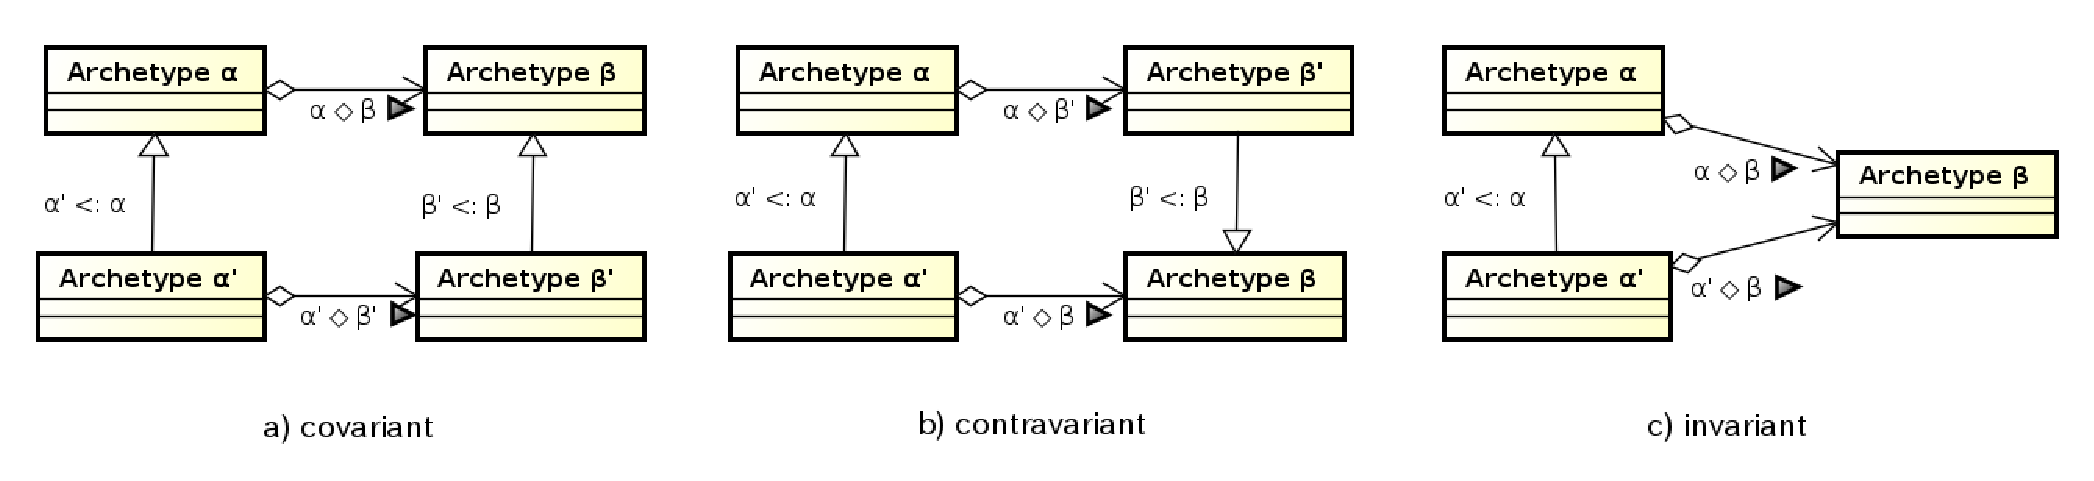
\includegraphics[width=16cm]{archetype_variance.eps}  
  \end{center}
  \caption{Three alternative archetype variances in a UML diagram}\label{fig:archetype_variances}
  {\footnotesize
    The figure shows three alternative archetype variances in a UML diagram. a) covariant: if $\alpha' <: \alpha$ and $\beta' <: \beta$, then $\alpha' \diamond \beta' <: \alpha \diamond \beta$, b) contravariant: if $\alpha' <: \alpha$ and $\beta' <: \beta$, then $\alpha' \diamond \beta <: \alpha \diamond \beta'$, and c) invariant: if $\alpha' <: \alpha$ and $\beta'= \beta$, then $\alpha' \diamond \beta <: \alpha \diamond \beta$.
    Note that, in this figure, the operator $<:$ denotes 'is a subtype of', and $\diamond$ denotes 'is composed of'.
    }
\end{figure*}

The actual variance of an archetype depends on the semantics of the archetype, i.e., how the archetype is constructed as a type. We consider this problem to be a major issue in archetype semantics because it affects the archetype expressiveness and extensibility as EHR schemas.

\begin{figure*}[!htbp]
a) covariant:

\begin{minipage}{0.49\linewidth}
\begin{Verbatim}[frame=single,fontsize=\small, commandchars=!\(\)]
archetype
  ISO-EN13606-COMPOSITION.alpha.v1


definition
  COMPOSITION[at0000] matches {
    !textit(content) matches {
      allow_archetype SECTION[at0001] matches {
        include
        archetype_id/value matches {
          "ISO-EN13606-SECTION.beta.v1"}}}}
\end{Verbatim}
\end{minipage}
\begin{minipage}{0.49\linewidth}
\begin{Verbatim}[frame=single,fontsize=\small, commandchars=!\(\)]
archetype
  ISO-EN13606-COMPOSITION.alpha-dash.v1
specialize
  ISO-EN13606-COMPOSITION.alpha.v1
definition
  COMPOSITION[at0000] matches {
    !textit(content) matches {
      allow_archetype SECTION[at0001] matches {
        include
        archetype_id/value matches {
          "ISO-EN13606-SECTION.beta-dash.v1"}}}}
\end{Verbatim}
\end{minipage}

b) contravariant:

\begin{minipage}{0.49\linewidth}
\begin{Verbatim}[frame=single,fontsize=\small, commandchars=!\(\)]
archetype
  ISO-EN13606-COMPOSITION.alpha.v1


definition
  COMPOSITION[at0000] matches {
    !textit(content) matches {
      allow_archetype SECTION[at0001] matches {
        include
        archetype_id/value matches {
          "ISO-EN13606-SECTION.beta-dash.v1"}}}}
\end{Verbatim}
\end{minipage}
\begin{minipage}{0.49\linewidth}
\begin{Verbatim}[frame=single,fontsize=\small, commandchars=!\(\)]
archetype
  ISO-EN13606-COMPOSITION.alpha-dash.v1
specialize
  ISO-EN13606-COMPOSITION.alpha.v1
definition
  COMPOSITION[at0000] matches {
    !textit(content) matches {
      allow_archetype SECTION[at0001] matches {
        include
        archetype_id/value matches {
          "ISO-EN13606-SECTION.beta.v1"}}}}
\end{Verbatim}
\end{minipage}

c) invariant:

\begin{minipage}{0.49\linewidth}
\begin{Verbatim}[frame=single,fontsize=\small, commandchars=!\(\)]
archetype
  ISO-EN13606-COMPOSITION.alpha.v1


definition
  COMPOSITION[at0000] matches {
    !textit(content) matches {
      allow_archetype SECTION[at0001] matches {
        include
        archetype_id/value matches {
          "ISO-EN13606-SECTION.beta.v1"}}}}
\end{Verbatim}
\end{minipage}
\begin{minipage}{0.49\linewidth}
\begin{Verbatim}[frame=single,fontsize=\small, commandchars=!\(\)]
archetype
  ISO-EN13606-COMPOSITION.alpha-dash.v1
specialize
  ISO-EN13606-COMPOSITION.alpha.v1
definition
  COMPOSITION[at0000] matches {
    !textit(content) matches {
      allow_archetype SECTION[at0001] matches {
        include
        archetype_id/value matches {
          "ISO-EN13606-SECTION.beta.v1"}}}}
\end{Verbatim}
\end{minipage}
  \caption{Examples of archetype variance in ADL}\label{fig:archetype_variances_adl}
\end{figure*}


\subsection{Typed lambda calculus}

In this section, we briefly introduce typed lambda calculus, which is the tool we use to investigate the archetype semantics. Lambda calculi are mathematical abstractions of computations, and in the typed lambda calculus, every variable must be explicitly typed. 
We herein use the terms typed lambda calculus and type theory interchangeably.

\subsubsection{How type theory is applied to ISO 13606}

Before introducing the details of the typed lambda calculus, we present an overview of the correspondence between the components of typed lambda calculus and ISO 13606.
In an abstract sense, a type is a well-defined set of values, so that every model in ISO 13606 can be encoded as a type.
Because each type has its own characteristics, we must carefully decide which types can be assigned to each component of ISO 13606.

We encoded unstructured RM components as primitive types in type theory.
Not surprisingly, a string in the RM is mapped to the string type. 
In contrast, structured RM components are mapped to structured types in type theory, such as record type, variant type, and list type.
For example, the TEXT type in ISO 13606 has charset, languages, and originalText as its field \cite[p.36]{iso08:13606_healt_elect_part1}.
Therefore, the TEXT type can be encoded as a record type using Eq.~\ref{eqn:text_as_record}.
Note that, in the present paper, concrete types, such as {\sf Record} or {\sf CS}, start with a capital letter and are shown in {\sf SansSerif} font.


\begin{figure*}[!htbp]
\begin{alignat}{3}
  \mathsf{TEXT} \equiv \mathsf{Record}\{charset \text{:} \mathsf{CS}, languages \text{:} \mathsf{CS}, originalText \text{:} \mathsf{String} \}  \label{eqn:text_as_record}
\end{alignat}
\end{figure*}

Archetypes, which are also structured, are encoded in record types.
For example, the vital signs archetype (Fig. \ref{fig:vital_signs_archetype}) can be encoded as shown in Eqs.~\ref{eqn:vital_signs_record} and \ref{eqn:vital_signs_section}.
The specialization of archetypes corresponds to Record subtyping, and the composition of archetypes corresponds to Record nesting.

\begin{figure*}[!htbp]
\begin{minipage}{1.0\linewidth}
\begin{Verbatim}[frame=single,fontsize=\small, commandchars=!\(\)]
!textit(definition)
   !textsf(SECTION)[at0000] matches {   -- Vital signs
      !textit(items) cardinality matches {2} matches {
         allow_archetype !textsf(OBSERVATION)[at0001] matches {
            include
               archetype_id/value matches {"openEHR-EHR-OBSERVATION.blood_pressure.v1"}
         }
         allow_archetype !textsf(OBSERVATION)[at0002] matches {
            include
               archetype_id/value matches {"openEHR-EHR-OBSERVATION.body_temperature.v1"}
         }
      }
   }
\end{Verbatim}
\end{minipage}
  \caption{Excerpt of a vital signs archetype} \label{fig:vital_signs_archetype}
  {\footnotesize
    This is an example of the definition section in a vital signs archetype.
    Note that we modified the certified archetype in the Clinical Knowledge Manager (CKM) repository to match the explanation herein.
    }
\end{figure*}


\begin{figure*}[!htbp]
\begin{alignat}{3}
  \mathsf{VitalSigns} & \equiv \mathsf{Record}\{&&definition[at0000] \text{:} \mathsf{SECTION^{VitalSigns}} \} && \label{eqn:vital_signs_record}\\
  \mathsf{SECTION^{VitalSigns}} & \equiv \mathsf{Record}\{&&items[at0001] \text{:} \mathsf{BloodPressure},\nonumber &&\label{eqn:vital_signs_section}\\
                              &                         &&items[at0002] \text{:} \mathsf{BloodTemperature}\}\} &&
\end{alignat}
\end{figure*}

EHR data are instances of Archetypes, \footnote{Note that this is not an "archetype instance", which is defined as a metadata class instance of an archetype model in the ISO 13606 specification \cite[p.2]{iso08:13606_healt_elect_part1}.} i.e., instances of the corresponding {\sf Record} type, because each EHR datum is created according to the corresponding archetype.
For example, Eq.~\ref{eqn:vital_signs_instance} represents an EHR datum for the vital sign archetype of Eq.~\ref{eqn:vital_signs_record}.
Note that instance names are written in lower case, e.g., $record$, and the details of $\mathsf{BloodPressure}$ and $\mathsf{BloodTemperature}$ are omitted for clarity in this equation.


\begin{figure*}[!htbp]
\begin{alignat}{3}
  vital\_signs \equiv record\{definition[at0000] \text{:} record\{&items[at0001] \text{:} record\{systolic\text{:} 120, diastolic \text{:} 80\},\nonumber\\
                                                                    &items[at0002] \text{:} record\{temperature\text{:} 37.5, unit \text{:} "C"\}\}\} \label{eqn:vital_signs_instance}
\end{alignat}
\end{figure*}

Table \ref{tab:correspondence} summarizes our assignment of ISO 13606 to type theory.
We believe that these assignments are intuitively plausible, as explained above.
However, this does not exclude other possibilities of assignments, which might lead to different results from those of the present study.

\begin{table}[!htbp]
  \centering
  \caption{Correspondence between type theory and ISO 13606}\label{tab:correspondence}
  \begin{tabular}{ccc}
    \toprule%[1.5pt]
    ISO 13606 & type theory \\
    \midrule
    primitive types in RM & basic types \\
    data structures in RM & structured types \\
    archetype & record type \\
    EHR data & instances of record type\\
    \bottomrule%[1.5pt]
  \end{tabular}
\end{table}


\subsubsection{Introducing types}

We next present the minimum set of typed lambda calculus that is sufficient to clarify the basis of archetype semantics (in particular variance and immutability of archetypes) by means of formalization in support of the aforementioned two assertions. 
We start from fundamental types, such as the function or basic type, and progressively extend the system with more complex types, such as the record or variant type (Table \ref{tab:types_notations}).
For a more comprehensive explanation of type theory, see for instance, \cite{pierce02:_types_progr_languag,cardelli04:_type_system,barendregt13:_lambd_calcul_types}.


\begin{table}[!htbp]
  \centering
  \caption{List of major types and corresponding notation used in the present study}\label{tab:types_notations}
  \vspace{6pt}
  \begin{tabular}{lcrr}
    \toprule %[1.5pt]
    type &  & notation \\
    \midrule
    function type &  & \(\tau \rightarrow \sigma \)\\
    basic types    &  & \(\mathsf{String}, \mathsf{Boolean}\), etc.\\
     &  \\
    & record type & \(\mathsf{Record}\)\\
    structured types & variant type & \(\mathsf{Variant}\)\\
    & list type & \([\tau]\)\\
    \bottomrule%[1.5pt]
  \end{tabular}
\end{table}

First, a formal assertion relating entities such as terms or types is referred to as a {\bf judgment} (Eq.~\ref{eqn:judgment}).
The judgment  $\Gamma ~ \vdash M:\tau$ should be read as "a term M has a type of $\tau$ under an environment $\Gamma$", and the judgment $\Gamma ~ \vdash \tau$ means that $\tau$ is a well-formed type under the environment $\Gamma$. In either case, $\Gamma$  is a set of assumptions about the types of free variables in $M$ and is referred to as the {\bf type environment}.
Note that, in the present study, we use M and N as terms, and $\tau$ and $\sigma$ for meta-variables over type.

\begin{alignat}{3}
  & {\Gamma~ \vdash \Omega} \qquad  \text{(judgment)}  \label{eqn:judgment}
\end{alignat}


In typed lambda calculus, types are introduced into the system by adding {\bf typing rules}, such as those given by Eq.~\ref{eqn:function_type_rule}.
These typing rules assert the validity of certain judgments based on other valid judgments.
The judgments above the horizontal line are referred to as the premises of the rule, and those below the horizontal line are referred to as the conclusion.

The most fundamental type is the Function Type ($\tau \rightarrow \sigma$), which satisfies the typing rule given by Eq.~\ref{eqn:function_type_rule}.
The notation $(M~N)$ in Eq.~\ref{eqn:application} denotes a function application in which a function $M$ is applied to the argument $N$.
A function is represented by a lambda abstraction, such as $\lambda x\text{:}\tau.M$ (Eqs.~\ref{eqn:lambda-abstraction_term} and \ref{eqn:lambda-abstraction_typing_rule}).
In this lambda abstraction, $x$ represents a parameter of the function, and $M$ represents the body of the function \cite[p.14]{cardelli04:_type_system}.
When we apply the term $M$ of function type $\tau \rightarrow \sigma$ to the value of type $\tau$, we obtain the term of type $\sigma$ (Eq.~\ref{eqn:application}).
This function type appears in database queries (such as Eq.~\ref{eqn:user_level_query}), because a query is a function that accepts a database and returns a result set of the database.

\begin{figure*}[!htbp]
  \begin{align}
        \text{Typing rules:} \qquad   \nonumber\\
    & \frac{\Gamma~ \vdash \tau \qquad \Gamma~ \vdash \sigma}
           {\Gamma~ \vdash \tau \rightarrow \sigma}  & \label{eqn:function_type_rule} \text{(function type)}\\[6pt]
    & \frac{\Gamma \vdash M\text{:}\tau \rightarrow \sigma \qquad  \Gamma \vdash N\text{:}\tau}
           {\Gamma ~ \vdash (M~N)\text{:}\sigma} & \qquad \text{(application)} \label{eqn:application}
  \end{align}
\caption{Function type and its application}
\end{figure*}

\begin{figure*}[!htbp]
\begin{alignat}{3}
  \text{Terms:} \qquad      & \nonumber\\
                               M~ & {::= } ~ \dots \\
                                  & | \quad {\lambda x\text{:}\tau.M} & \qquad (\lambda~abstraction) \label{eqn:lambda-abstraction_term}\\
  \text{Typing rule:} \qquad &       & \nonumber \\
                              & \frac{\Gamma,x\text{:}\tau~ \vdash M\text{:}\sigma }
                                      {\Gamma ~ \vdash \lambda x\text{:}\tau.M\text{:}\tau \rightarrow \sigma} & \label{eqn:lambda-abstraction_typing_rule}
\end{alignat}
\caption{$\lambda$ abstraction}\label{eqn:lambda-abstraction}
\end{figure*}

Because EHR data are aggregates of various types of data, we need to introduce such data types.
For example, blood pressure data are constructed as aggregates with the numeric type for the pressure value and a string type for the unit of measurement.
We classify these data types into two categories: basic and structured.
Basic types, such as Boolean or Integer,  are primitive data types in that they lack any internal structure.
When these primitive types are built in BasicType, they are available in our system as Eq.~\ref{eqn:basic_type_rule}.
$\Gamma~ \vdash \diamond$ means that $\Gamma$ is well-typed, which means that the type environment $\Gamma$ has nothing but valid types.
  
\begin{figure}[!htbp]
  \begin{align}
    \frac{\Gamma~ \vdash \diamond \qquad \tau \in \mathsf{BasicType}}
    {\Gamma~ \vdash \tau} \label{eqn:basic_type_rule}
  \end{align}
\end{figure}

ISO 13606 provides several kinds of primitive types, such as {\sf String} and {\sf Boolean} \cite[p.42]{iso08:13606_healt_elect_part1}.
For example, the {\sf Boolean} type can be introduced into the proposed type system by Eq.~\ref{eqn:basic_type_rule}, because $\mathsf{Boolean} \in \mathsf{BasicType}$ holds in ISO 13606.
As one such primitive type, we introduce the {\sf{\bf Unit}} type (Eq.~\ref{eqn:type_unit}), which has no corresponding type in ISO 13606.
The Unit type has only one value called {\it{unit}} (Eq.~\ref{eqn:unit_typing_rule}), which is often used as a filler for uninteresting results \cite{cardelli04:_type_system,pierce02:_types_progr_languag}.
In the present paper, this type is used in a field of Variant type (Eq.~\ref{eqn:type_hepatitis}) and a return value of assignments (Eq.~{\ref{eqn:assignment}}).


\begin{figure*}[!htbp]
\begin{alignat}{3}
  \text{Types:} \qquad   \nonumber\\
                        \tau~ & {::= \dots }\nonumber\\
                              & | ~~ \mathsf{Unit}                                & \qquad \label{eqn:type_unit} \text{(type unit)}\\
  \text{Typing rules:} \qquad   \nonumber\\
                              & \frac{\Gamma~ \vdash \diamond }
                                      {\Gamma ~ \vdash unit \text{:}\mathsf{Unit}} & \label{eqn:unit_typing_rule} \text{(value unit)}
\end{alignat}
\caption{Unit}\label{fig:unit_type}
\end{figure*}

EHR data are inherently structured in that they consist of large collections of data entities of several types.
Thus, we introduce such structured data types into our type system in order to capture the ISO 13660 data model.
These structured types are Record, Variant, and List types.
  
\begin{enumerate}
\item Record Type

  A {\sf{\bf Record}} type is a cross-product of the values with a projection operation for extracting components by name \cite[p.18]{cardelli04:_type_system,pierce02:_types_progr_languag}.
  As stated previously, most of the components in archetypes, such as Fig. \ref{fig:vital_signs_archetype}, are encoded as {\sf Record} types (Eqs.~\ref{eqn:vital_signs_record} and \ref{eqn:vital_signs_section}).

  The definition of structured type has three sections. In the record type, the terms section defines syntactic forms of a record and its projection (Eqs.~\ref{eqn:record_construction} and \ref{eqn:record_projection}). The types section defines the $\mathsf{Record}$ type itself (Eq.~\ref{eqn:record_type}). And, the typing rules section defines rules for the type of record construction and its projection (Eqs.~\ref{eqn:record_constructiontyping_rule} and \ref{eqn:record_projection_typing_rule}). Note that $i \in 1..n$ is shorthand for $\{ i~|~ i  \in \mathbb{N} \wedge 1 \leq i \wedge i \leq n )\}$, which indicates that the variable $i$ ranges over natural numbers $\mathbb{N}$ from 1 to $n$.
Also note that a record is basically a tuple, the components of which are not indexed by numbers but rather labeled by names. Therefore, the components in {\sf{Record}} type are unordered.

\begin{figure*}[!htbp]
    \begin{alignat}{4}
        \text{Terms:} \qquad   \nonumber\\
        M~ & {::= \dots }\nonumber\\
           & | ~~ record\{l_i = M\} \qquad where~i \in 1..n & (\text{record construction}) \label{eqn:record_construction}\\
           & | ~~M.l_i    & (\text{record projection}) \label{eqn:record_projection}\\
        \text{Types:} \qquad   \nonumber\\
        \tau~  & {::= \dots}\nonumber\\
               &  |~~ \mathsf{Record}\{l_i \text{:} \tau_i \} \qquad where~i \in 1..n \label{eqn:record_type}\\
        \text{Typing rules:} \qquad   \nonumber\\
        & \frac{\Gamma \vdash M_i\text{:}\tau_i}
               {\Gamma ~ \vdash record\{l_i\text{:} M_i\}: \mathsf{Record}\{l_i \text{:} \tau_i\}} \qquad where~i \in 1..n \label{eqn:record_constructiontyping_rule} \\[6pt]
        & \frac{\Gamma \vdash M \text{:} \mathsf{Record}\{l_i \text{:} \tau_i\}}
               {\Gamma ~ \vdash M.l_i \text{:} \tau_i} \qquad where~i \in 1..n \label{eqn:record_projection_typing_rule}
     \end{alignat}
     \caption{Records}\label{fig:record_type}
\end{figure*}   

\item Variant Type
  
  While {\sf Record} type requires all of the fields to be set by values, there is a case in which only one of the fields must be filled in. 
  This is called the ${\sf{\bf Variant}}$ Type, which is a named disjoint union of types \cite[p.136]{pierce02:_types_progr_languag}\cite[p.19]{cardelli04:_type_system}.
  Figure \ref{fig:example_variant_type} is an example of such a case, and this fragment of the archetype should be encoded as a variant type (Eqs.~\ref{eqn:value_hepatitis} and \ref{eqn:type_hepatitis}).

\begin{figure*}[!htbp]
\begin{alignat}{3}
  \text{Terms:} \qquad   \nonumber\\
                        M~& {::= \dots } \nonumber\\
                          & | ~~ variant\langle l_i = M_i \rangle \qquad where~i \in 1..n & (\text{variant construction}) \label{eqn:variant_construction}\\
                          % & | ~~ \text{case}~M~\text{of}~\langle  l_i = x_i \rangle ~\Rightarrow~ M_i \qquad where~i \in 1..n  & (\text{variant case match}) \label{eqn:variant_case_match}\\
  \text{Types:} \qquad   \nonumber\\
                        \tau~ & {::= \dots} \nonumber\\
                              & |~~ \mathsf{Variant}\langle  l_i \text{:} \tau_i \rangle \qquad where~i \in 1..n \\
  \text{Typing rules:} \qquad   \nonumber\\
                           & \frac{\Gamma \vdash M_j\text{:}\tau_j \qquad where~i \in 1..n}
                                  {\Gamma ~ \vdash variant\langle l_j\text{:} M_j\rangle: \mathsf{Variant}\langle l_i \text{:} \tau_i\rangle^{i \in 1..n} } \label{eqn:variant_constructiontyping_rule} \\[6pt]
                                  % & \frac{\Gamma \vdash M \text{:} \mathsf{Variant}\langle l_i\text{:} \tau_i\rangle \qquad \Gamma,x_i\text{:}\tau_i ~\vdash M_i \text{:} \tau} 
                                  % {\Gamma ~ \vdash \text{case}~M~\text{of}~\langle  l_i = x_i \rangle ~\Rightarrow~ M_i\text{:}\tau}  \qquad where~i \in 1..n 
\end{alignat}
\caption{Variants}\label{fig:variant_type}
\end{figure*}


\begin{figure}[!htbp]
\begin{minipage}{1.0\linewidth}
\begin{Verbatim}[frame=single,fontsize=\small, commandchars=!\(\)]
       !textit(value) matches {
           !textsf(DV_CODED_TEXT) matches {
             !textit(defining_code) matches {
               [local::
                at1000,  -- Hepatitis A
                at1001   -- Hepatitis B
               ]
             }
          }
      }
\end{Verbatim}
\end{minipage}
  \caption{Example of a Variant Type in DV\_CODED\_TEXT}\label{fig:example_variant_type}
  {\footnotesize
    This fragment defines a constraint of type DV\_CODED\_TEXT, the value of which should be either hepatitis A or B.
  }
\end{figure}

\begin{figure*}[!htbp]
  \begin{alignat}{3}
    value & : \mathsf{DV\_CODED\_TEXT^{HepatitisVirus}} \label{eqn:value_hepatitis}\\
    \mathsf{DV\_CODED\_TEXT^{HepatitisVirus}} & \equiv \mathsf{Record}\{defining\_code \text{:} \mathsf{Variant}\langle \text{at1000} \text{:} \mathsf{Unit},~\text{at1001} \text{:} \mathsf{Unit} \rangle\} \label{eqn:type_hepatitis}
  \end{alignat}
\end{figure*}

\item List Type

  EHR data sometimes contain a series of events, such as a sequence of laboratory data in the context of hemodialysis. These kinds of collective values are represented by the {\sf{\bf List}} type \cite{cardelli04:_type_system,pierce02:_types_progr_languag,geuvers09:_introd_type_theor}.
  In the present paper, the {\sf List} type is denoted by $[\tau]$, describing finite-length sequences the element of which are taken from $\tau$.
  Figure \ref{fig:example_list_type} is an example of such a case, and the {\it{parts}} attribute in this fragment of the archetype should be encoded as a {\sf List} type (Eq.~\ref{eqn:type_parts}).


\begin{figure*}[!htbp]
\begin{minipage}{1.0\linewidth}
\begin{Verbatim}[frame=single,fontsize=\small, commandchars=!\(\)]
!textit(definition)
   !textsf(CLUSTER) [at0000] matches {
      !textit(parts) cardinality matches {0..*; ordered} matches {
         allow_archetype !textsf(ENTRY) matches {
            include
               archetype_id/value matches {
                  "CEN-EN13606-ENTRY.laboratory.v1"
               }
         }
      }
   }
\end{Verbatim}
\end{minipage}
  \caption{Example of a List Type in CLUSTER}\label{fig:example_list_type}
\end{figure*}

\begin{figure*}[!htbp]
  \begin{alignat}{3}
    definition & \text{:} \mathsf{CLUSTER^{Haemodialysis}}\\
    \mathsf{CLUSTER^{Haemodialysis}} & \equiv \mathsf{Record}\{parts \text{:} [\mathsf{LaboratoryEntry}]\} \label{eqn:type_parts}
  \end{alignat}
\end{figure*}

\end{enumerate}


\subsubsection{Subtyping}

EHR data are organized hierarchically.
In Fig. \ref{fig:excerpt_reference_model}, for example, {\sf ELEMENT} and {\sf CLUSTER} are subordinate to {\sf ITEM} in their hierarchy, because each subordinate class (i.e., {\sf ELEMENT} and {\sf CLUSTER}) inherits all of the members of its parent class {\sf ITEM}.
This hierarchical relation, which is implemented as inheritance in object-oriented languages, is formalized as {\bf subtyping} in type theory \cite[p.85]{craig07:_objec_orien_progr_languag}.
In this section, we introduce general rules for subtyping and specific rules for each type.
When we define the specific subtyping rules so as to be compatible with the general rules, we are able to check the validity of a given subtyping based on a deductive system of the type theory.

\begin{figure}[!htbp]
  \begin{center}
    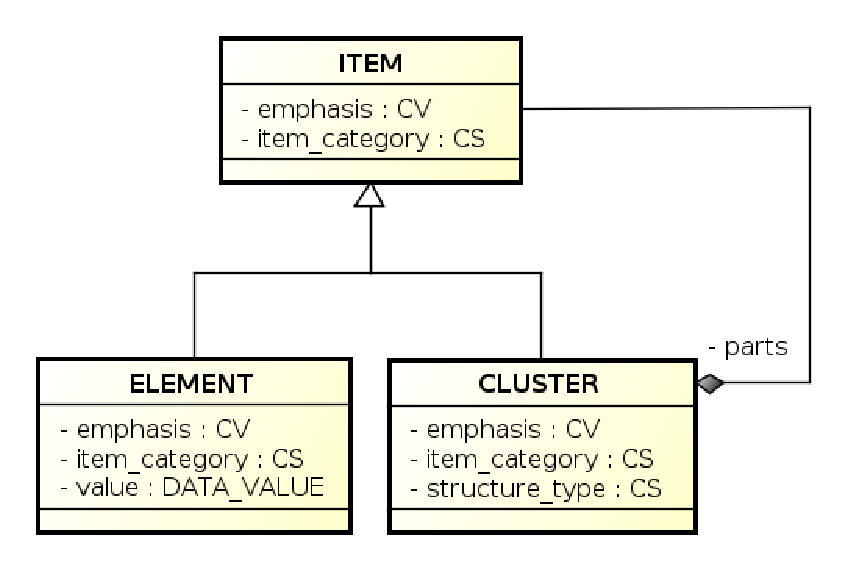
\includegraphics[width=6cm]{excerpt_reference_model.eps}  
  \end{center}
  \caption{Excerpt of the ISO 13606 Reference Model}\label{fig:excerpt_reference_model}
  {\footnotesize
    This UML diagram is an excerpt from the ISO 13606 Reference Model \cite[p.10]{iso08:13606_healt_elect_part1} and defines the hierarchy of {\sf ITEM} and its subordinates {\sf ELEMENT} and {\sf CLUSTER}.
    }
\end{figure}

The central theorem of subtyping is the {\bf subsumption principle} (Eq.~\ref{eqn:subsumption_rule}), which says that if type $\tau'$ is a subtype of $\tau$ (i.e., $\tau' <: \tau$), then an instance of type $\tau'$ can be used in any context in which an instance of type $\tau$ can appear.
Note that the subtyping operator '$<:$' is a reflexive transitive closure (Eqs.~\ref{eqn:subtyping_reflexive} and \ref{eqn:subtyping_transitive}) similar to the numeric comparison operator '$\leq$', so that  $\tau' <: \tau \text{ and}~ \tau <: \tau' $ means that $\tau \text{ is equal to } \tau'$ (cf., $a \leq b \text{ and}~ b \leq a $ means that $a = b$).

\begin{figure*}[!htbp]
\begin{alignat}{2}
        \text{Typing rules:} \qquad   \nonumber\\
        & \frac{\Gamma~ \vdash M \text{:} \tau'  \qquad \Gamma~ \vdash \tau' <: \tau}
               {\Gamma~ \vdash M \text{:} \tau} & \text{(subsumption principle)}\label{eqn:subsumption_rule}\\[6pt]
        & \frac{\Gamma~ \vdash \tau}
               {\Gamma~ \vdash \tau <: \tau} & \label{eqn:subtyping_reflexive} \text{(reflexive)}\\[6pt]
        & \frac{\Gamma~ \vdash \tau'' <: \tau' \qquad \Gamma~ \vdash \tau' <: \tau}
               {\Gamma~ \vdash \tau'' <: \tau} & \label{eqn:subtyping_transitive} \text{(transitive)}
\end{alignat}
\end{figure*}


Subtyping rules should be defined for each type, and every subtyping rule should be compatible with the subsumption principle.
We next present the subtyping rules for structured types. 
In the record type, one record type is a breadth subtype of another if the first has at least all of the fields of the second (Eq.~\ref{eqn:record_width_subtyping}), and the other record type is a depth subtype of another if they have exactly the same fields, but the types of the corresponding fields are subtypes (Eq.~\ref{eqn:record_depth_subtyping}).
In the variant type, the depth subtyping rule for the variant type is identical to that of the record type (cf., Eqs.~\ref{eqn:variant_depth_subtyping} and \ref{eqn:record_depth_subtyping}), but the breadth subtyping rules for the variant type is different from that for the record type: a subtype of the variant type cannot have more fields than its supertype (Eq.~\ref{eqn:variant_breadth_subtyping}).
The variance of the list type is defined as covariant, as in the case of the {\sf Record} type. Therefore, in the case of a list having elements of type $\tau'$, and $\tau' <: \tau$, we can regard the list as having elements of type $\tau$ (Eq.~{\ref{eqn:list_subtyping_rule})} \cite[p.197]{pierce02:_types_progr_languag}.

Since we abstracted archetypes as record types, archetype specialization can be modeled as record subtyping. We can add new items or modify the existing items in the specialized archetype as long as the extensions are compatible with Eqs.~\ref{eqn:record_width_subtyping} and \ref{eqn:record_depth_subtyping}.

\begin{figure*}[!htbp]
  \begin{alignat}{3}
    \text{Record subtyping rules:} \qquad   \nonumber\\
    & \frac{\Gamma \vdash \tau_i \qquad where~i \in 1..n+m} 
           {\Gamma ~ \vdash \mathsf{Record}\{l_i \text{:} \tau_i\}_{i \in 1..n+m}  <: \mathsf{Record}\{l_i \text{:} \tau_i\}_{i \in 1..n}}  & \label{eqn:record_width_subtyping}\\[6pt]
    & \frac{\Gamma \vdash \tau'_i <: \tau_i}
           {\Gamma ~ \vdash \mathsf{Record}\{l_i\text{:}\tau'_i \}  <: \mathsf{Record}\{l_i\text{:}\tau_i\}}  \qquad where~i \in 1..n & \label{eqn:record_depth_subtyping}\\
    \text{Variant subtyping rules:} \qquad   \nonumber\\
    & \frac{\Gamma \vdash \tau_i \qquad where~i \in 1..n+m} 
           {\Gamma ~ \vdash \mathsf{Variant}\langle l_i\text{:} \tau_i\rangle_{i \in 1..n}  <: \mathsf{Variant}\langle l_i\text{:}\tau_i\rangle_{i \in 1..n+m}}  & \label{eqn:variant_breadth_subtyping}\\[6pt]
    & \frac{\Gamma \vdash \tau'_i <: \tau_i}
           {\Gamma ~ \vdash \mathsf{Variant}\langle l_i\text{:}\tau'_i \rangle  <: \mathsf{Variant}\langle l_i\text{:}\tau_i\rangle}  \qquad where~i \in 1..n & \label{eqn:variant_depth_subtyping}\\
    \text{List subtyping rule:} \qquad   \nonumber\\
    & \frac{\Gamma \vdash \tau' <: \tau}
           {\Gamma ~ \vdash [\tau'] <: [\tau]}                                                    & \label{eqn:list_subtyping_rule}
  \end{alignat}
  \caption{Subtyping rules for Record, Variant, and List}\label{fig:subtyping_rules_record_variant_list}
\end{figure*}

Structured types, even basic types, can be subtyped by introducing an ad hoc subtyping rule \cite[p.28]{cardelli04:_type_system}.
When we define the ad hoc rules, their actual characteristics of the values should be compatible with the subsumption principle. Otherwise, the system is consistent in theory, but useless in reality.
For example, since an integer value can be used in the context in which a real value can appear (e.g., 1 as 1.0), a subtyping rule $\mathsf{Integer} <: \mathsf{Real}$ can be introduced.
This can also be applied to the structured types in the RM, as long as they are compatible with the ISO 13606 specification. According to Fig. \ref{fig:excerpt_reference_model}, for example, we can define subtyping between {\sf ELEMENT} and {\sf ITEM} as shown in Eq.~\ref{eqn:element_subtyping} and {\sf CLUSTER} and {\sf ITEM} as shown in Eq.~\ref{eqn:cluster_subtyping}.

\begin{alignat}{3}
  \frac{\Gamma~ \vdash \diamond}
       {\Gamma~ \vdash \mathsf{ELEMENT} <: \mathsf{ITEM}} \qquad \text{(ad-hoc)} \label{eqn:element_subtyping} \\[6pt]
  \frac{\Gamma~ \vdash \diamond}
       {\Gamma~ \vdash \mathsf{CLUSTER} <: \mathsf{ITEM}} \qquad \text{(ad-hoc)} \label{eqn:cluster_subtyping}
\end{alignat}



\subsubsection{Type system and its deductive system}

Deductive proofs are necessary in order to confirm the validity of the assertions under a given system.
When we define a number of type rules based on previous disciplines, the collection of axioms and typing rules is referred as a {\bf type system}.
Once we have a type system, we can construct a deductive proof by combining the typing rules, and the proof is referred to as a {\bf derivation tree}.
Any derivation tree has leaves at the top and a root at the bottom, where each judgment is obtained from those immediately above it by applying some of the rules of the system.
Figure \ref{fig:example_derivation_tree} shows a simple example of a derivation tree, indicating that the function of type $\mathsf{String} \rightarrow \mathsf{Integer}$ yields an integer type when applied to a string value. Note that the number in brackets to the right of the horizontal line indicates the equation number of the rule that was used (in this case, {Eq.~\ref{eqn:application}}).
This deductive proof system is the most powerful feature of typed lambda calculus, because we can investigate the semantics of ISO 13606 with formal deductions. 


%\begin{pf}
\begin{figure*}[!htbp]
\begin{prooftree}
  \AxiomC{$\Gamma ~ \vdash \lambda x$:$\mathsf{String}.M$:$\mathsf{String} \rightarrow \mathsf{Integer}$}
  \AxiomC{$\Gamma ~ \vdash "text"$:$\mathsf{String}$}
  \RightLabel{[\ref{eqn:application}]}
  \BinaryInfC{$\Gamma ~ \vdash ((\lambda x$:$\mathsf{String}.M)~"text") $:$ \mathsf{Integer}$}
\end{prooftree}
\caption{An example of a derivation tree}\label{fig:example_derivation_tree}
\end{figure*}
%\end{pf}

\subsection{Application of type theory to ISO 13606}

In the previous sections, we introduced basic components of type theory and the correspondence of type theory to ISO 13606.
Next, we need to encode the problems in terms of this formal language in order to support the assertions (Assertions 1 and 2). 

\subsubsection{How to formalize queries \label{sec:howto_formalize_queries}}

{\bf Assertion 2}, which states that ``data created with any specialized archetype will always be matched by queries based on the parent archetype'', is related to a requirement as to which queries and specialization should be obeyed.
Before deriving the assertion from the proposed type system, we encoded this assertion in terms of typed lambda calculus as follows.

Database theories \cite{hillebrand96:_datab_query_languag_embed_typed_lambd_calcul,grust99:_compr_queries,grust99:_how_compr_queries_funct,poulovassilis96:_algeb} tell us that the database can be presented as list of data, and its queries can be encoded as lambda terms and {\tt foldr} (Eqs.~\ref{eqn:database_as_list} and \ref{eqn:query_by_foldr}).
Note that archetype is abbreviated as $\alpha$, N is a database containing a list of EHR data created by archetype $\alpha$, and $[~]$ is an empty list.
The database query has function type, because Eq.~\ref{eqn:query_by_foldr} indicates that $query~p$ takes a database that consists of a list of data (i.e., $[\alpha]$) and returns a result that also consists of a list of data (i.e., $[\alpha]$). The lambda term $p$ in Eq.~\ref{eqn:user_level_query} is a user-level query that is applied to each element of a collection, as {\tt{foldr}} calls itself recursively. The essential logic of query is embedded in term M. For instance, if we define $p \equiv \lambda x\text{:}\alpha.(\lambda xs\text{:}[\alpha].(\text{if}~ x.id == \text{"blood~pressure"} ~\text{then}~ x\text{:}xs ~\text{else}~ xs))$, then $query~p~N$ filters out the list of data for which the id field is "blood pressure".

\begin{figure*}[!htbp]
\begin{alignat}{3}
   database \equiv & ~ N \text{:} [\alpha] \label{eqn:database_as_list}\\
   query~p  \equiv & ~ \mathtt{foldr} ~ p ~[~] \text{:} [\alpha] \rightarrow [\alpha] \label{eqn:query_by_foldr}\\
           & \text{where}  \quad   p \equiv \lambda~x\text{:}\alpha.(\lambda~xs\text{:}[\alpha].M) \text{:} \alpha \rightarrow [\alpha] \rightarrow [\alpha] \label{eqn:user_level_query} \quad \text{and,}\\
                  & \qquad   \text{{\tt foldr} is a higher-order combinator for recursion \cite{hutton99:tutorial_universality_expressiveness_fold,bird92:_introd_funct_progr}} \nonumber
\end{alignat}
\end{figure*}


Based on these preconditions, {\bf Assertion 2} is formally expressed in Fig. \ref{fig:formalized_second_assertion}. The next task is to derive the judgment $(query~p)~N' \text{:} [\alpha] $ from these premises to support {\bf Assertion 2}.

\begin{figure}[!htbp]
\begin{alignat}{3}
  \text{provided that\quad}   & \Gamma \vdash \alpha' <: \alpha \text{, and}~ \\
                              & \Gamma \vdash query~p\text{:}[\alpha] \rightarrow [\alpha]\text{, and}~ \\
                              & \Gamma \vdash  N'\text{:}[\alpha'] \\
  \text{then, derive\quad} & \Gamma \vdash (query~p)~N' \text{:}[\alpha] ~ & 
\end{alignat}
\caption{Assertion 2 formalized}\label{fig:formalized_second_assertion}
\end{figure}


\subsubsection{How to introduce assignments for EHR data \label{sec:howto_introduce_assignments}}

Thus far, it has been impossible to update EHR data, because the record type, for example, has only the projection operation and not the assignment operation for updating (Eq.~\ref{eqn:record_projection}).
Most programming languages and database systems, however, use destructive updating methods. In other words, old values are replaced by new values. 
Regarding this issue, an archetype is said to be mutable if a reference of the value can be obtained and updated by the assignment. Otherwise, it is said to be immutable, because the value cannot be mutated \cite[p.295]{harper13:_pract_found_progr_languag}.
We attempted to change archetypes from immutable to mutable by introducing update functionality, and investigated what would happen to the archetype semantics.

In order to represent mutable archetypes, an additional type called the {\sf{\bf Ref}} type must be introduced. 
The value of the {\sf Ref} type is a reference that designates the mutable locations in memory \footnote{Interested readers can refer to Pierce \cite[p.159]{pierce02:_types_progr_languag} or Bruce \cite[p.77]{bruce02:_found_objec_orien_languag} for more concrete explanations.}, described as $\mathsf{Ref(\tau)}$ (Eq.~\ref{eqn:type_reference}). 
If term M has type $\mathsf{Ref(\tau)}$, then M denotes a location that can hold a value of type $\tau$. 
A datum can be updated by assignment operator ':=', the return type of which is {\sf Unit} type (Eqs.~\ref{eqn:type_unit} and \ref{eqn:assignment}).

\begin{figure*}[!htbp]
\begin{alignat}{3}
  \text{Types:} \qquad   \nonumber\\
                        \tau~ & {::= \dots }\\
                              & | ~~ \mathsf{Ref(\tau)}                           & \qquad \label{eqn:type_reference} \text{(type reference)}\\
  \text{Typing rules:} \qquad   \nonumber\\
                              & \frac{\Gamma~ \vdash M\text{:}\mathsf{Ref(\tau)} \qquad \Gamma~ \vdash N\text{:}\tau}
                                      {\Gamma ~ \vdash M := N\text{:}\mathsf{Unit}} & \label{eqn:assignment} \qquad\qquad \text{(assignment)}\\
  \text{Subtyping rules:} \qquad   \nonumber\\
                              & \frac{\Gamma ~ \vdash \tau' <: \tau \qquad \Gamma ~ \vdash \tau <: \tau'}
                                     {\Gamma ~ \vdash \mathsf{Ref(\tau')} <: \mathsf{Ref(\tau)}} \label{eqn:reference_subtyping}
\end{alignat}
\caption{Reference Type}\label{fig:reference_type}
\end{figure*}

Thus, the mutable archetype itself is encoded as $\mathsf{Archetype}\{l_i \text{:} \mathsf{Ref}(\tau_i)\}$ \cite[p.19]{cardelli04:_type_system}, and the typing rule of the archetype is given by Eq.~\ref{eqn:mutable_record_field_reference}, which indicates that the subtyping relation of mutable Archetype depends on the subtyping of the {\sf Ref} type. 
  Note that the {\sf Ref} type must be taken to be invariant in order to preserve type safety (Eq.~{\ref{eqn:reference_subtyping}}). This restrictive subtyping rule is necessary because a value of type {\sf Ref} can be used in a context of both reading and writing \cite[p.198]{pierce02:_types_progr_languag}\cite[p.29]{cardelli04:_type_system}.

In the Results section , we describe a critical change in the archetype semantics that is brought about by this new encoding of the archetype.

\begin{alignat}{3}
  & \frac{\Gamma \vdash M_i \text{:} \mathsf{Ref}(\tau_i) }
         {\Gamma ~ \vdash archetype\{l_i\text{:} M_i\} \text{:} \mathsf{Archetype}\{l_i \text{:} \mathsf{Ref}(\tau_i) \} } ~~ (i \in 1..n) \label{eqn:mutable_record_field_reference}
\end{alignat}


\section{Results}


Based on the basic semantics of ISO 13606 archetypes , we derived two assertions (Assertions 1 and 2) in this section.
Moreover, we investigated the consequences of introducing mutable archetypes and clarified the effects of this introduction on the archetype semantics.

\subsection{Archetypes should follow the subsumption principle}

We derived {\bf Assertion 1}, which states that any data created via the use of a specialized archetype shall be conformant both to the specialized archetype and its parent archetype as follows.
We divided this assertion into two cases: 1) any data created via an archetype shall be conformant to itself, and 2) any data created via the specialized archetype shall be conformant to its parent archetype.
Assume an archetype is abbreviated as $\alpha$ and a specialized archetype is abbreviated as $\alpha'$, then we get  $\alpha' <: \alpha$.
Hence, the first case is straightforward because we have a trivial equality of $M \text{:} \alpha = M \text{:} \alpha$.
The second case is also straightforward. If archetypes are encoded as Record types and follow the subsumption principle, then the second case states the subsumption principle itself (cf., Eq.~\ref{eqn:subsumption_rule}).


\subsection{Archetypes should be covariant}

In Section \ref{sec:variances_archetype}, we encountered three alternatives of variance when we combined archetypes by both specialization and composition.
By defining the archetypes as $\mathsf{Archetype}\{l_i \text{:} \tau_i \}$ and combining subtyping rules for record type (Eqs.~\ref{eqn:record_width_subtyping} and \ref{eqn:record_depth_subtyping}), we obtain the subtyping rule for archetypes as Eq.~\ref{eqn:archetype_subtyping}, which reveals that archetypes are covariant in their components.

  \begin{alignat}{3}
    & \frac{\Gamma \vdash \tau'_i <: \tau_i \qquad where~i \in 1..n+m}
           {\Gamma ~ \vdash \mathsf{Archetype}\{l_i\text{:} \tau'_i \}_{i \in 1..n+m}  <: \mathsf{Archetype}\{l_i\text{:} \tau_i\}_{i \in 1..n}}   & \label{eqn:archetype_subtyping}
  \end{alignat}

Once the variance of archetypes is fixed as covariant, this affects not only the underlying semantics but also the syntax of the archetype slot. Suppose that an archetype composes another archetype with a regular expression $\text{/openEHR-EHR-CLUSTER.device.*/}$ in the archetype slot and that its specialized archetype composes the other archetype with \verb|/*/|. In this case, any data, even if the data are a supertype of the CLUSTER-device, can be set to the field, which violates the covariant requirement. Therefore, we claim that every composed archetype should be uniquely specified in the archetype slot by an exact archetype identifier, such as that shown in Fig. \ref{fig:archetype_slot_in_string}. In addition, we do not have to explicitly exclude improper archetypes, because they are implicitly excluded if they are not subtypes of the specified archetype.

\begin{figure*}[!htbp]
\begin{minipage}{1.0\linewidth}
\begin{Verbatim}[frame=single,fontsize=\small, commandchars=!\(\)]
            !textsf(ITEM_TREE)[at0011] matches {
                !textit(items) matches {
                    allow_archetype matches {
                        include
                            archetype_id/value matches {"openEHR-EHR-CLUSTER.device.v1"}
                    }
                }
            }
\end{Verbatim}
\end{minipage}
\caption{An example of a uniquely identified archetype slot}\label{fig:archetype_slot_in_string}
{\footnotesize
  In this fragment of ADL, the archetype 'openEHR-EHR-CLUSTER.device.v1' is identified as a string in the archetype slot, and so is uniquely specified.
  }
\end{figure*}



 \subsection{Queries should be reusable}

Assertion 2 insists that queries should be reusable.
We define a number of archetypes at a certain point in time, and the data are stored in the EHR system based on the defined archetypes.
As time passes, some of the archetypes are specialized to create more detailed archetypes, as in Fig. {\ref{fig:cohort_study}}. New EHR data, which are conformant to the specialized archetypes, will accumulate in the system.
Then, it is natural to want to run the queries defined on the first generation archetypes on the EHR data that are conformant to their specialized archetypes.
This is what Assertion 2 demands.

In Section \ref{sec:howto_formalize_queries}, we formalized Assertion 2 in terms of typed lambda calculus, as shown in Fig. \ref{fig:formalized_second_assertion}.
The formalized statement of the assertion was used to derive $(query~p)~N' \text{:}[\alpha]$ from the assumptions $\alpha' <: \alpha, query~p\text{:}[\alpha] \rightarrow [\alpha]$, and $N'\text{:}[\alpha']$.
Note that $\alpha$ is a parent archetype, $\alpha'$ is the specialized archetype of $\alpha$, and $N' \text{:} [\alpha']$ refers to ``a list of data created by the specialized archetype $\alpha'$''.
This is case A in Fig. \ref{fig:archetype_queries}, because we are applying a query for a parent archetype $\alpha$ to the data created from its specialized archetype $\alpha'$.
Given these conditions, we constructed the following derivation tree to support Assertion 2 (Fig. \ref{derivation_second_assertion}).


\begin{figure*}[!htbp]
  \begin{center}
    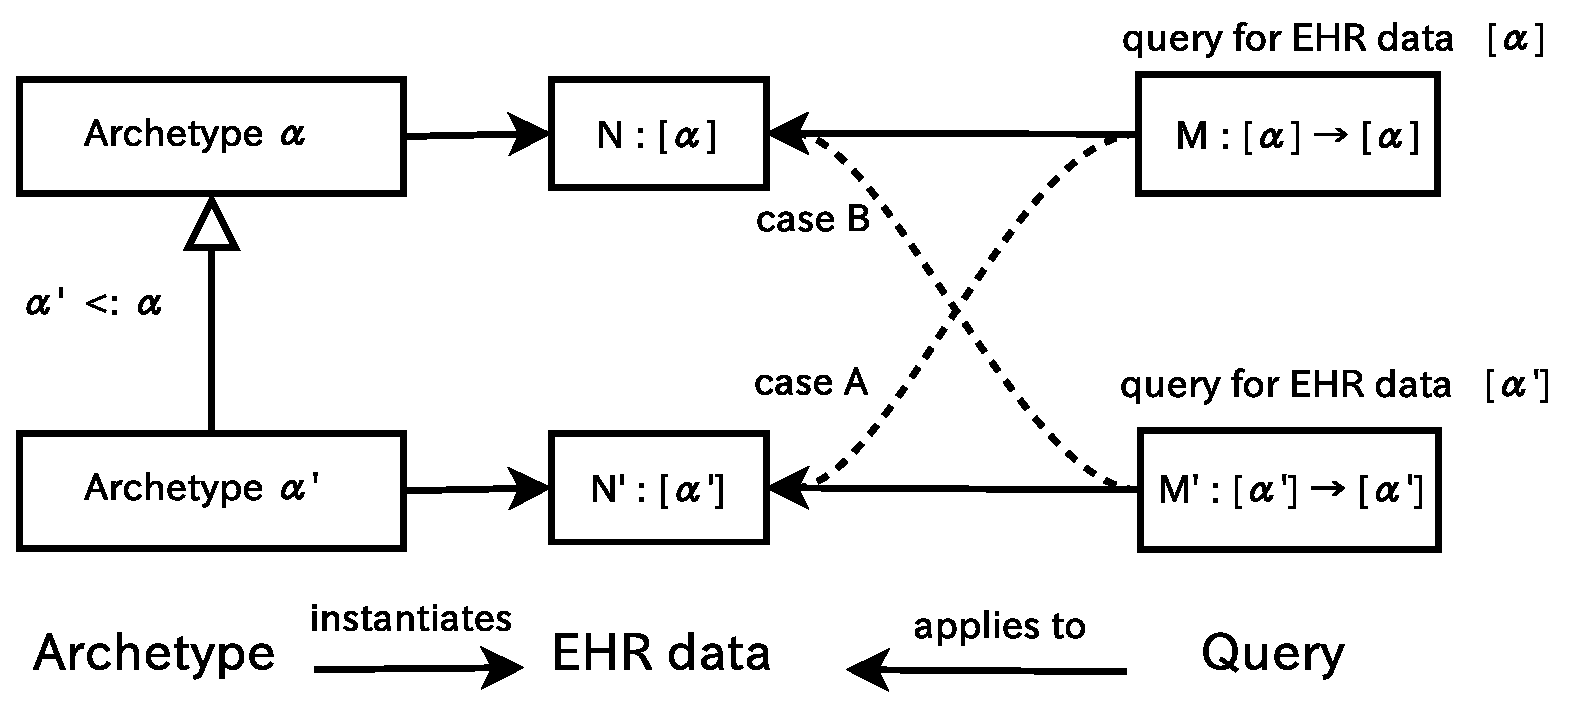
\includegraphics[width=10cm,clip]{archetype_based_queries.eps}  
  \end{center}
\caption{Two cases of query applications}\label{fig:archetype_queries}
{\footnotesize
  This figure describes the relationships between archetypes, EHR data, and their queries. Four arrows are drawn from queries to EHR data. The two solid arrows indicate ordinary queries, the argument type of which is matched to the type of the EHR data (e.g., $M\text{:}[\alpha] \rightarrow [\alpha]$ and $N\text{:}[\alpha]$). The two dotted arrows indicate the cases for which we investigated the validity in the text.
  }
\end{figure*}


%\begin{pf}
\begin{figure*}[!htbp]
\begin{prooftree}
  \AxiomC{$\Gamma~ \vdash \alpha' <: \alpha$}
  \RightLabel{\quad [\ref{eqn:list_subtyping_rule}]}
  \UnaryInfC{$\Gamma~ \vdash [\alpha'] <: [\alpha]$}
  \AxiomC{$\Gamma~ \vdash N'\text{:} [\alpha']$}
  \RightLabel{\quad [\ref{eqn:subsumption_rule}]}
  \BinaryInfC{$\Gamma~ \vdash N'\text{:} [\alpha]$}
  \AxiomC{$\Gamma~ \vdash query~p \text{:} [\alpha] \rightarrow [\alpha]$}
  \RightLabel{\quad [\ref{eqn:application}]}
  \BinaryInfC{$\Gamma~ \vdash (query~p)~N'\text{:}[\alpha]$}
\end{prooftree}\caption{Derivation of Assertion 2}\label{derivation_second_assertion}
\end{figure*}
%\end{pf}


The significance of this derivation is not so clear. Therefore, we presented the opposite case of applying a query for the specialized archetype $\alpha'$ to the data from the parent archetype $\alpha$. This assumption corresponds to case B in Fig. \ref{fig:archetype_queries}.
In this case, the query is encoded as $M' \text{:} [\alpha'] \rightarrow [\alpha']$, and the target database is encoded as $N\text{:}[\alpha]$. Then, it is obvious that $(M'~N)$ causes a type error, because $[\alpha']$ does not match $[\alpha]$ (cf., Eq.~\ref{eqn:application}). This indicates that the queries based on the parent archetype are applicable to the data created by its specialized archetype whereas queries based on a specialized archetype are not applicable to data created with the parent archetypes.

\subsection{Archetypes should be invariant if they are mutable schema}

Section \ref{sec:howto_introduce_assignments} revealed that if we want to update EHR data, we must encode Archetype as $\mathsf{Archetype}\{l_i\text{:} \mathsf{Ref}(\tau^i) \}$ as in Eq.~\ref{eqn:mutable_record_field_reference}. Therefore, we need to determine how to derive the judgment $\mathsf{Archetype}\{l\text{:} \mathsf{Ref(\tau')} \}  <: \mathsf{Archetype}\{l\text{:} \mathsf{Ref(\tau)}\}$ based on the modified type system.

Since subtyping of {\sf Ref} types is defined in Eq.~\ref{eqn:reference_subtyping}, we derived the tree shown in Fig. \ref{fig:derivation_mutable_archetype} by combining the mutable Archetype judgment and the {\sf Ref} subtyping rules.

%\begin{pf}
\begin{figure}[!htbp]
\begin{prooftree}
  \AxiomC{$\tau' <: \tau$}
  \AxiomC{$\tau <: \tau'$}
  \RightLabel{\quad [\ref{eqn:reference_subtyping}]}
  \BinaryInfC{$\mathsf{Ref(\tau')} <: \mathsf{Ref(\tau)}$}
  \RightLabel{\quad [\ref{eqn:archetype_subtyping}]}
  \UnaryInfC{$\mathsf{Archetype}\{l\text{:} \mathsf{Ref(\tau')} \}  <: \mathsf{Archetype}\{l\text{:} \mathsf{Ref(\tau)}\}$}
\end{prooftree}\caption{Derivation of the mutable archetype}\label{fig:derivation_mutable_archetype}
\end{figure}
%\end{pf}

Figure \ref{fig:derivation_mutable_archetype} shows that subtyping of mutable archetypes depends on the type of $\tau$ and $\tau'$. However, $\tau' <: \tau \text{ and}~ \tau <: \tau' $ means that $\tau \text{ is equal to } \tau'$, because subtyping operator $<:$ is both transitive and reflexive (Eqs.~\ref{eqn:subtyping_reflexive} and \ref{eqn:subtyping_transitive}). Therefore, the derivation of Fig. \ref{fig:derivation_mutable_archetype} reveals that archetypes must be invariant if they are mutable archetypes.


Since this consequence is less intuitive, it is demonstrated through a counterexample. Based on Eq.~\ref{eqn:hypothesis}, let us assume that mutable archetypes are covariant. Then, we identify an inconsistency from this false hypothesis.

\begin{figure*}[!htbp]
\begin{alignat}{3}
  \text{Typing rules:} \qquad   \nonumber\\
    & \frac{\Gamma \vdash \tau'_i <: \tau_i  \qquad where~i \in 1..n+m}
           {\Gamma ~ \vdash \mathsf{Archetype}\{l_i\text{:} \mathsf{Ref(\tau'_i)} \}_{i \in 1..n+m}  <: \mathsf{Archetype}\{l_i\text{:} \mathsf{Ref(\tau_i)}\}_{i \in 1..n}} \label{eqn:hypothesis}
\end{alignat}
\end{figure*}

Provided that type $\mathsf{Int}$ is integer and type $\mathsf{PosInt}$ is a positive integer, we assert that $\mathsf{PosInt} <: \mathsf{Int}$ by ad hoc rule, and suppose that $\mathsf{Archetype^A}\{l\text{:}\mathsf{Ref(PosInt)}\}$ and $\mathsf{Archetype^B}\{l_1\text{:} \mathsf{Ref(Int)}\}$. 

Then, since we assume the mutable Archetype to be covariant, $\mathsf{Archetype^A} <: \mathsf{Archetype^B}$ should hold (Eq.~\ref{eqn:hypothesis}). In addition, let us define $a \equiv archetype\{l = 1\} \text{:} \mathsf{Archetype^A}$ and $b \equiv archetype\{l = -1\} \text{:} \mathsf{Archetype^B}$. Given these settings, we can derive $a.l := -1$ as in Fig. \ref{fig:derivation_mutable_archetype_covariant}. This, however, contradicts $a.l \text{:} \mathsf{Ref(PosInt)}$, because $-1$ is {\it not} a positive integer.


%\begin{pf}
\begin{figure*}[!htbp]
\begin{prooftree}
  \AxiomC{$\mathsf{PosInt} <: \mathsf{Int}$}
  \RightLabel{\quad [\ref{eqn:hypothesis}]}
  \UnaryInfC{$\mathsf{Archetype^A} <: \mathsf{Archetype^B}$}
  \AxiomC{$a$:$\mathsf{Archetype^A}$}
  \RightLabel{\quad [\ref{eqn:subsumption_rule}]}
  \BinaryInfC{$a\text{:}\mathsf{Archetype^B}$}
  \RightLabel{\quad [\ref{eqn:record_projection}]}
  \UnaryInfC{$a.l\text{:}\mathsf{Ref(Int)}$}
  \AxiomC{$-1 \text{:} \mathsf{Int}$}
  \RightLabel{\quad [\ref{eqn:assignment}]}
  \BinaryInfC{$a.l := -1 \text{:} \mathsf{Unit}$}
\end{prooftree}\caption{Derivation from the false hypothesis}\label{fig:derivation_mutable_archetype_covariant}
\end{figure*}
%\end{pf}

As described above, if we allow EHR data to be updatable, then the semantics of the archetype is modified, and the variance of archetypes is changed from covariant to invariant.

\subsection{Archetypes should be both covariant and immutable}


Thus far, we have obtained different consequences of archetype variance from different premises. If the archetype is immutable, then the archetype is covariant, otherwise the archetype is invariant.
Both consequences are valid in terms of type theory.
As previously explained in Section \ref{sec:higher_concepts}, we need higher concepts than the type theory to decide which consequence is more appropriate. 
These higher concepts were 'structural interoperability' and 'schema extensibility'.


For the case in which the archetype is covariant, we can construct a specialized archetype along with its composition. 
Looking back at the aforementioned schema in Fig. {\ref{fig:cohort_study}}, it should be noted that the schema is composed in a completely covariant manner.
When we specialize the {\sf RevisedCase} from the {\sf InitialCase}, we can also specialize its composition outcome from {\sf InitialOutcome} to {\sf RevisedOutcome}. For the case in which the archetype is invariant, we cannot specialize the components of the parent archetypes. Although structural interoperability is still guaranteed in this case, schema extensibility is severely restricted. Comparing these two alternatives, we conclude that, for the sake of schema extensibility, the archetype should be immutable.


\subsection{EHR data are safe\label{sec:ehr_data_safety}}

EHR data are created, validated, and queried based on their corresponding archetypes. We defined the basic semantics of archetypes - in particular variance and immutability of archetypes -  in terms of the type system, and we clarified the behaviors of the semantics in terms of the derivations. However, we only inferred these derivations by symbolic manipulations referred to collectively as deduction and did not perform any evaluation such as queries or projections.
Finally, a simple question remains: Aren't there any discrepancies between the results from the deductions and the values of the EHR data from the actual evaluation results?
The answer lies in a property of the type theory.

A carefully constructed type system can take advantage of a property called {\bf soundness}.
If a type system is sound, then every derived judgment in the system is assured to be valid, so that the system is free from type errors \cite{mitchell00:_found_progr_languag,cardelli04:_type_system}.
This is the fundamental requirement of structural interoperability, because if you cannot perform a computation on some data but obtain an error, the EHR system can never be operated safely.

The soundness is stated in a more formal manner \cite[p.12]{cardelli04:_type_system} by Eq.~\ref{eq:soundness}, which indicates that if M is an instance type $\tau$ (i.e., $M\text{:}\tau$), then M will be evaluated to obtain a value that has an inferred type of $\tau$.
Note that $\llbracket {~} \rrbracket$ is a function that evaluates a lambda term to obtain its value when applied to the term or infers the type of the term to obtain its simpler type when applied to the type itself.

\begin{equation}
  \label{eq:soundness}
  \text{if} ~~ \Gamma \vdash M \text{:} \tau ~~\text{is valid, then}~~ \llbracket M \rrbracket \in \llbracket \tau \rrbracket ~\text{holds.}
\end{equation}

Note that the aforementioned type system is sound \cite{gunter92:_seman_progr_languag,wright94:_syntac_approac_to_type_sound}, i.e., Eq.~\ref{eq:soundness} holds for every component of the proposed type system. We omit the soundness proof, because it is beyond the scope of the present paper \footnote{Interested readers can refer to Fisher \cite{fisher94:_lambd_calcul_objec_method_special} or Wright \cite{wright94:_syntac_approac_to_type_sound} for a complete reference on the proof.}. Instead, we present an example in which the soundness holds.

Suppose term M is a projection function from $\mathsf{Archetype}\{l \text{:} \mathsf{TEXT}\}$ to $\mathsf{TEXT}$ (Eq.~\ref{eqn:example_evaluation_M_type}) and N is an instance of that archetype (Eq.~\ref{eqn:example_evaluation_N_type}). Then, the evaluation of the term $(M~N)$ produces the value "text" from Eq.~\ref{eqn:evaluation_application}. On the other hand, when we infer the type of (M N), we obtain $\mathsf{TEXT}$ (Fig. \ref{fig:example_type_inference}).
Looking at the results of evaluation in both the term and the type, it is obvious that $"text" \in \mathsf{TEXT}$ holds.

\begin{figure*}[!htbp]
\begin{alignat}{3}
\text{provided that,} \quad  M & \equiv \lambda x\text{:}\mathsf{Archetype}\{l \text{:} \mathsf{TEXT}\}.(x.l) \text{:} \mathsf{Archetype}\{l \text{:} \mathsf{TEXT}\} \rightarrow \mathsf{TEXT} \label{eqn:example_evaluation_M_type}\\
                             N & \equiv archetype\{l = "text"\} \text{:} \mathsf{Archetype}\{l \text{:} \mathsf{TEXT}\} \label{eqn:example_evaluation_N_type}\\
\text{then,} \quad             \llbracket (M~N) \rrbracket & \Rightarrow_{\beta} "text" \label{eqn:evaluation_application}\\
                              & \text{where } \Rightarrow_{\beta}  \text{is called $\beta$-conversion that does } (\lambda x.M) N \Rightarrow_{\beta} M[x := N] \nonumber
\end{alignat}\caption{Evaluation of a lambda term $(M~N)$ }\label{fig:example_evaluation}
\end{figure*}

%\begin{pf}
\begin{figure*}[!htbp]
\begin{prooftree}
  \AxiomC{$M \text{:} \mathsf{Archetype}\{l\text{:} \mathsf{TEXT}\} \rightarrow \mathsf{TEXT}$}
  \AxiomC{$N \text{:} \mathsf{Archetype}\{l \text{:} \mathsf{TEXT}\}$}
  \RightLabel{\quad [\ref{eqn:application}]}
  \BinaryInfC{$(M~N) \text{:} \mathsf{TEXT}$}
\end{prooftree}\caption{Type inference of a lambda term $(M~N)$}\label{fig:example_type_inference}
\end{figure*}
%\end{pf}

Although this is a small example, Eq.~\ref{eq:soundness} holds for every component, even for larger components such as EHR data, as long as the system is sound.
Then, we are justified in saying that the proposed sound type system guarantees the conformance of EHR data to their archetypes and that EHR data are safe in terms of type theory.

\section{Discussion}

In the present paper, we assigned major components of ISO 13606 to their proper types and derived multiple results for variance from different premises of mutability, using a deductive system of the type theory. As a result, we reached the conclusion that the archetype should be a covariant and immutable schema. Furthermore, we redefined the method of composing an archetype as uniquely designating the target archetype in an archetype slot.

In this section, we explain the importance of formal semantics, and discuss the assets and limitations of typed lambda calculus as compared with other formal methodologies that have been used in related research.

\subsection{Why formal semantics is needed}

The primary reason we could reach the above conclusion is that we built the basic formal semantics of ISO 13606.
However, some readers might suspect that the primary subject of the standard is message modeling of EHR Extract, and such a conceptualized semantics is considered to be beyond the scope of the standard.
Indeed, the purpose of ISO 13606 is stated as follows:
\begin{quote}
  ISO 13606 may offer a practical and useful contribution to the design of EHR systems but will primarily be realized as a common set of external {\it interfaces} or {\it messages} \cite[v]{iso08:13606_healt_elect_part1}.
\end{quote}

Despite this fact, we insist that semantics is an indispensable part of the standard and should be thoroughly investigated.

In informatics, the term 'message' implies a grammatical arrangement of words rather than a substantial internal structure or behaviors. The validity of messages, however, depends not only on the grammar but also the semantics: an underlying principle for the internal structure and behavior. For example, "Plato loved Socrates" is a sensible sentence, whereas "Friday hates Saturday" is not, even though this sentence is grammatically correct. In other words, messages must conform to semantics, as well as to grammar. In these examples, the semantics is a constraint that restricts the domain of the function 'love' or 'hate' to human beings. It is semantics that underpins the validity of messages.

Semantics, despite its significance, is invisible, and thus appears unfamiliar. We can literally see the phrase "Plato loved Socrates" as an alphabetic sequence, but the function of 'love' itself, let alone its domain, is unclear. However, once we formalize the semantics, they can be visualized. When every term and rule is defined as a symbol, then inference can be seen as an arrangement of symbols, just as a sentence can be seen as an arrangement of words. Then, we can easily explore the semantics: the inference mechanism rigorously excludes invalid results and derives novel results that could never be foreseen. In terms of the degree to which they are conceptualized, this mechanism is similar to the laws of physics, which capture the true nature of the world as mathematical symbols and greatly expand the boundaries of our knowledge.

\subsection{Implication of  formal semantics}


The purpose of building the system of physics is to model the natural phenomena in a general and reproducible manner so that future phenomena, such as solar eclipses, can be predicted.
Then, for what purpose is our formal semantics built?
If there is no practical purpose, then the present study is merely an empty manipulation of abstract symbols, and there will be no contribution to medical informatics.

As previously stated in Section {\ref{sec:ehr_data_safety}}, the purpose of these formal semantics is the analysis of the ISO 13606 specification, so that only safe operations on EHR data are permitted and all erroneous operations are denied in terms of type system.  
In contrast, if data or type safety is not assured in the specification, then the EHR system will cause errors in the long run.
The disaster of NASA's Mars Climate Orbiter in 1999 is a good example of such a failure of data management, because the root cause was a ``failure to use metric units in the coding of a ground software file'' {\cite{stephenson99:_mars_climat_orbit_mishap_inves_board}}.
A numerous system failures ,which rooted in Java's null pointer exceptions, has been occurring in the course of ordinary operations on earth.
This kind of runtime exception occurs when the null value reference {\footnote{The null value is a reference that does not point to anything.}} is accessed.
We can get rid of these errors in advance if we introduce proper types for each value based on a sound type system.
Therefore, the implication of the present study, which is building engines for next-generation EHR systems devoid of data management failures, is rather practical.


\subsection{Assets of typed lambda calculus}

We used typed lambda calculus as the formalization methodology, and there are several reasons why we chose this formalism.

First, typed lambda calculus has a long history of research in computer science as the computational model of statically typed programming languages. The theory laid the ground for not only typed functional languages, such as ML and Haskell, but also for object-oriented languages, such as Java \cite{igarashi01:_feath_java,barendregt13:_lambd_calcul_types}.
Second, type theory as a formalized deductive system is useful for proof-theoretic investigations \cite[p.9]{program13:_homot_type_theor}. We can construct proofs of already defined typed rules by properly combining the rules. Furthermore, the validity of the proofs depends only on the syntactic aspects thereof. This property of the theory helps us to check the proof, as we did in the present paper.
Third, the soundness of the type system ensures the validity of the consequences derived from the proof. If a value is proved to belong to a type, then the value must be exactly that type. This indicates that we can avoid erroneous operations of an EHR system that is built upon a sound archetype repository.

Thus, typed lambda calculus guarantees a certain type of interoperability - we call it structural interoperability - based on these properties. The knowledge and disciplines are so abstract and general that the results can be applied not only to ISO 13606, but also to every other standard in pursuit of the same goal.


\subsection{Related research}

We found two basic types of related research on formal semantics of archetypes. One type uses regular grammar theory \cite{jose09:_linkeh_ed,maldonado07:_framew_for_clinic_data_stand_based_archet}, and the other type uses Description Logic (DL) \cite{martinez-costa08:_model_driven_approac_for_repres,maldonado12:_using_resear_ehr,lezcano11:_integ_owl_swrl,martinez-costa10:_iso_en_openeh,costa12:_towar}.

Maldonado et al. \cite{jose09:_linkeh_ed,maldonado07:_framew_for_clinic_data_stand_based_archet} attempted to construct formal semantics of archetypes by means of regular grammar theory.  They abstracted archetypes as a tree with labeled nodes and developed a type system based on the concept of a constrained multiplicity list. They chose this approach because the functionality of archetypes resembles that of XML Schema, and the use of the regular grammar theory has been successful in building a formal theory of XML Schema \cite{chidlovskii00:_using_regul_tree_autom_xml,murata05:_taxon_of_xml_schem_languag}. These papers explained the semantics of archetype specialization and conformance of EHR data but did not investigate the issues of archetype variance or mutability as we did in the present study.

Several studies took a different approach, such as transferring archetypes to OWL, and these studies used DL, which is widely used as a theoretical foundation of ontology. 
Whereas most of the studies \cite{martinez-costa08:_model_driven_approac_for_repres,maldonado12:_using_resear_ehr,lezcano11:_integ_owl_swrl,martinez-costa10:_iso_en_openeh,costa12:_towar} simply translated archetypes to OWL, Marcos et al. \cite{menarguez-tortosa13:_owl} performed DL reasoning to check the consistency of archetypes, and they found out that  22.2\% of the archetypes in the Clinical Knowledge Manager (CKM) repository and 21.2\% of the archetypes in the National Health Service (NHS) repository were inconsistent. 
The study, however, has a weaknesses.
Although they took into account compositions through archetype slots in checking the consistency of specialization, it was unclear which variance of archetypes was assumed to be true in the reasoning.
It was presumed to be covariant only after the following citation was found: "The specialized archetype uses the datatype {\sf{DV\_TEXT}} instead of {\sf{CODED\_TEXT}}\footnote{Note that {\sf{CODED\_TEXT}} is a subtype of {\sf{DV\_TEXT}} (i.e., $\mathsf{CODED\_TEXT} <: \mathsf{DV\_TEXT}$) in openEHR specification \cite[p.21]{beale08:_refer_model_data_types_infor_model}.}" \cite[p.312]{menarguez-tortosa13:_owl}.
In addition, they provided no theoretical ground for this assumption, so that they had no choice but to overlook the issue of archetype variance or immutability that was intensively analyzed by typed lambda calculus in our study.

As a matter of fact, intuitionistic logic and typed lambda calculus are deeply related as indicated by the Curry-Howard isomorphism \cite{lawler08:_class_logic_curry_howar_corres,sorensen98:_lectur_curry_howar_isomor}.
The main idea here is that a logical formula can be interpreted as types in a type theory, and the proof of a formula is associated with a lambda term of the proper type. As a result, if a formula is derivable in a logical system, then the corresponding type is inhabited in the type theory \cite{asperti91:_categ_types_and_struc}.
This correspondence also seems to hold between DL and a type theory, because some DLs can be thought of as notational variants of certain propositional modal logics \cite[p.38]{baader07:_descr_logic_handb}\cite{rijke98:_modal_logic_descr_logic}, and a certain type theory is known to have the same expressiveness as modal logic \cite{nanevski05:_contex_model_type_theor}.

Even though there is some correspondence between DL and type theory, we insist that type theory is a more suitable methodology than DL for the purpose of the present study. Being a logical framework for knowledge representation, DL is capable of checking the consistency of defined semantics, but is incapable of deriving theorems from axioms and rules. On the other hand, type theory is a theory, the formal definition of which is a set of formulas that is closed under logical consequence \cite[p.32]{ben-ari12:_mathem_logic_comput_scien}. These theories are constructed by selecting a set of formulas called axioms (e.g., typing rules) and deducing their logical consequences, which are called theorems (i.e., derivation trees).
In investigating a formal semantics of a specification, it is crucial to define axioms and to derive the logical consequences of the axioms, i.e., theorems, in order to determine whether these axioms and theorems fit with the requirements of the specification.
We chose type theory instead of DL, because the chosen theory is more suitable for the investigation of semantics.

\subsection{Limitations}

We chose typed lambda calculus as a formal methodology and have clarified some important aspects of archetype semantics that have been overlooked in previous studies. Despite these achievements, there are some limitations in this formalism. Specifically, whether type theory, which is inherently conservative due to its soundness, can cover the entire range of ISO 13606 archetype semantics remains unknown. Moreover, there are some difficult issues in encoding Archetype.

First, variant types prevent a schema from being extended, because its subtype has fewer choices than its supertype (Eq. \ref{eqn:variant_breadth_subtyping}). Suppose that we wanted to store a history of hepatitis and, therefore, developed an archetype in which the choice of hepatitis is expressed as a variant type. Only hepatitis A and B were known to us at the time the archetype was developed. Therefore, we encoded the two alternatives as CODED\_TEXT.defining\_code (Fig. \ref{fig:example_variant_type}). Later, a problem was encountered when hepatitis C was discovered. Since the subtype of a variant type has fewer choices than the supertype (Eq.~\ref{eqn:variant_breadth_subtyping}), we cannot specialize the existing archetype. In order to avoid this inconvenience, we must define a new archetype that contains three types of hepatitis, namely, hepatitis A, B, and C. However, this approach does not involve extending the schema, but rather creating an additional schema, which is not reusable for existing queries, as shown in Fig. \ref{derivation_second_assertion}.


Second, it is difficult to encode an archetype model in which fields are parametrized by the RM type. Even though we have shown how to express Archetype in typed lambda calculus, we intentionally ignored the fact that the field name of Archetype is partly dependent on the type of RM \cite[p.63]{iso08:13606_healt_elect_part2} and instead hard-coded the structure as a Record type. For example, archetypes having an RM type of SECTION, such as $\text{CEN-EN13606-SECTION.substance\_use}$, should have a members field, whereas an archetype having an RM type of ENTRY, such as CEN-EN13606-ENTRY.substance\_use, should have items and meaning fields. These fields cannot be parametrized according to the defined type system. Even if we attempt to introduce higher-order types \cite[p.24]{cardelli04:_type_system}, such attempts fail because the higher-order types parametrize only types and not the associated field names. This type of parametrized archetype is thought to be very difficult to encode in any existing formalisms, including the regular grammar theory or DL.

Third, we did not discuss attribute constraints, such as cardinality, existence, occurrences, order, unique, and multiple-valued attributes \cite[p.83-84]{iso08:13606_healt_elect_part2}.
The cardinality and occurrences constraints are difficult to handle in this simple type theory, because they are expressed as intervals, such as $\{0..1\}$ or $\{10..*\}$.
In the case of multiple-valued attributes, the constraints are also difficult to handle.
The multiple-valued attributes are constrained by an instance of C\_MULTIPLE\_ATTRIBUTE, which allows multiple
co-existing member objects of the container value of the attribute to be constrained \cite[x]{iso08:13606_healt_elect_part2}.
Figure \ref{fig:guitar_example} shows an example of multiple-valued attributes. This {\it{parts}} attribute will be encoded as a {\sf{List}} type, but its element type cannot be determined, because it contains two items.

\begin{figure*}[!htbp]
\begin{minipage}{1.0\linewidth}
\begin{Verbatim}[frame=single,fontsize=\small, commandchars=!\(\)]
 definition
   !textsf(INSTRUMENT)[at0000] matches {
     !textit(size) matches {|60..120|}
     !textit(date_of_manufacture) matches {yyyy-mm-??}
     !textit(parts) cardinality matches {0..*} matches {
       !textsf(PART)[at0001] matches { -- neck
          !textit(material) matches {
             [local::at0003]  -- timber
          }
       }
       !textsf(PART)[at0002] matches { -- body
          !textit(material) matches {
             [local::at0003]  -- timber
          }
       }
    }
 }
\end{Verbatim}
\end{minipage}
\caption{Excerpt of the guitar archetype \cite[xvi]{iso08:13606_healt_elect_part2}}\label{fig:guitar_example}
\end{figure*}
  

\subsection{On Exactitude in Science}

As stated in the previous section, the present study has several limitations, and therefore we cannot claim to have achieved full formal semantics of ISO 13606 based on the proposed type system.
Nevertheless, we insist that building a formal semantics of archetypes, even if it is incomplete, is of fundamental importance.

The activity of modeling or abstraction is to focus on the essential part of the subject while discarding the subtle details for some purposes. 
For example, a map that describes only highways and ignores small lanes can be useful for specific purposes, such as driving between big cities.
On the other hand, a map that describes every detail of geographical information will become gigantic, and may be useless as a map (c.f., Jorge Luis Borges's ''On Exactitude in Science'' \cite{borges99:_collec_jorge_luis_borges}).
A more suitable example in computer science is Featherweight Java (FJ) \cite{igarashi01:_feath_java},
which is a formal semantics of Java's type system based primarily on typed lambda calculus.
Even though the semantics did not cover the full semantics of the Java programming language, it provided a significant boost to the enrichment of the language with advanced features, such as generic class or inner class \cite[p.246]{pierce02:_types_progr_languag}.
It is often meaningful to build a formal semantics that is less complete but more compact, offering sufficient insight for minimum investment.

In the analysis of the present study, we have dealt with the type constraint, omitting attribute constraints, as described above.
While our formal semantics was less complete, we obtained important insights on the variance and mutability of archetypes.
Moreover, we cannot add new types or typing rules that would contradict the already defined type system, otherwise the soundness of the system will be lost.
Therefore, as long as we take our type theory as a solid basis for the foundation of archetype semantics, these insights are expected to be valid even if we enrich the proposed type system to handle other constraints.
Returning to the map metaphor, although we can draw a more detailed map by adding small lanes, these lanes would never override existing highways.


\subsection{Prospectives}

As mentioned above, the proposed type theory did not cover the entire range of ISO 13606 archetype semantics, because the type theory we introduced was too simple.
We believe that the coverage of the proposed theory can be widened if we add more type rules or extend the type system by adding more advanced features.

First, bulk data structures, such as a list or a set, in ISO 13606 are parametrized according to the type of its elements, as in modern programming languages \cite[p.42]{iso08:13606_healt_elect_part1}.
These types can be correctly captured, if we introduce a recursive type to the proposed system \cite{cardelli04:_type_system,geuvers09:_introd_type_theor}.
  
Second, we did not discuss attribute constraints as stated previously.
The order and unique constraints, however, can be handled together so that we can determine a suitable type for each container. As the specification indicates \cite[p.84]{iso08:13606_healt_elect_part2}, the proper collection type can be assigned according to the combination of order and unique constraints.
An existence constraint can be also handled if we introduce the $\mathsf{Option}$ type, which represents optional values \cite[p.137]{pierce02:_types_progr_languag}.


Third, although ISO 13606 attempts to represent every conceivable type of health record data structure in a consistent manner \cite[vi]{iso08:13606_healt_elect_part1}, the unit of measurement is a major exception, because the units are expressed only as string representations, e.g., kg or mmHg \cite[p.46,p.82]{iso08:13606_healt_elect_part2}, not as a structured data type. This makes it difficult to properly convert or calculate EHR data according to their units. Type theory can address this problem when the units are constructed as a type \cite{kennedy94:_dimen_types,kennedy10:_types_units_measur}. Once we develop that kind of type system with sound semantics, we can manipulate EHR data in a more consistent manner, for example, by automatic unit conversion or dimension-based validation.

These examples suggest that if we add more advanced features, we can enrich the semantics and extend the interoperability of ISO 13606 even beyond the reach of the original scope of the standard. In the future, we intend to encode and analyze the semantics of the ISO 13606 archetype with the latest results for the theory.


\section{Conclusions}

For ISO 13606, a solid foundation is necessary for the archetype semantics in order to achieve structural interoperability between EHR systems.
We analyzed the semantics by a formal methodology based on typed lambda calculus and clarified the following:

\begin{enumerate}
\item Archetypes should be both covariant and immutable schema, so that the structural interoperability is guaranteed and EHR schema are extended over time.
\item An archetype should uniquely specify other archetypes in the archetype slot when they are composed.
\end{enumerate}

We hope that the results of the present study will provide all who are involved in ISO 13606 with a measure of insight and suggestions for the renewal tasks of the standard. 

\section*{Acknowledgments}

The authors would like to thank Ms.~Mirai Ikebuchi for her advice on mathematical notation and for checking our derivations and Mr.~Yasuhide Miura for his assistance in preparing the manuscript.

The present study was supported in part by the Japan Society for the Promotion of Science (JSPS) through the Funding Program for World Leading Innovative R\&D on Science and Technology (FIRST program).

%\bibliographystyle{elsarticle-num-names}
\bibliographystyle{vancouver}
\bibliography{books}

\end{document}

%%% Local Variables: 
%%% mode: japanese-latex
%%% TeX-master: t
%%% End: 











